\chapter{Analýza}
Cílem této kapitoly je analyzovat entity, procesy a fungování projektu a postupně sestavit funkční a nefunkční požadavky na výslednou aplikaci. Na základě toho pak může být započat návrh jednotlivých částí aplikace.
    
    \section{Procesy a entity}
    V této sekci popíši fungování projektu, které rozdělím do několika částí, resp. entit. Vzhledem k tomu, že se v projektu pohybuje jediný člověk, lektorka, a tato aplikace slouží jako podpůrný prvek procesů v projektu (tedy např. neřeší objednání klienta, to proběhne např. telefonicky, osobně, e-mailem, pouze zaznamenává potřebná data a umožňuje s nimi pracovat a zobrazovat tak, aby zefektivnila jednotlivé procesy), je upuštěno od modelování procesů ve prospěch podrobného textového popisu, na základě kterého bude vytvořen co nejpřesnější návrh této aplikace.
    
        \subsection{Kurzy}\label{subsec:kurzy}
        ÚP nabízí v současné době 6 kurzů, plánují se ale i další, stejně tak ale některé mohou být ukončeny. Každý kurz má svůj název. Jsou individuální a skupinové, neexistuje ale žádná přímá souvislost mezi kurzem a způsobem jeho výuky, protože se vše přizpůsobuje na míru klientovi, tedy některý kurz může sice být obvykle vyučován skupinově, ale někdy také individuálně. Mají variabilní délku, většinou od 1 měsíce až po celoroční. Všechny kurzy jsou placené a většinou je na rodičích, zda zaplatí celý kurz, platí měsíčně, každou lekci, nebo úplně individuálně (platí se v hotovosti nebo převodem). Konají se ve všední dny, v současné době 3x týdně od odpoledne až do večera. Na kurz se klient objednává telefonicky, e-mailem, zprávou nebo osobně.
        
        \subsection{Klienti}\label{subsec:klienti}
        Účastník kurzu se nazývá klient. Kurzy navštěvuje buď sám za sebe, tedy individuálně, nebo je součástí nějaké skupiny (viz. následující podsekce~\ref{subsec:skupiny}). U klienta je potřeba evidovat jméno a příjmení, e-mailový a telefonní kontakt na rodiče a případně další poznámky. Vzhledem k tomu, že v současné době byla evidence používána v podobě uvedené v sekci~\ref{aktualni-reseni}, často některé kontaktní údaje schází a je třeba s tím počítat.
        
        \subsection{Skupiny}\label{subsec:skupiny}
        Zejména v poslední době se v projektu zvyšuje počet skupinových lekcí. Skupinu tvoří většinou 2 až 4 klienti, kteří v rámci této skupiny dochází na příslušný kurz. Lektorka pro lepší orientaci skupinám vytváří jejich jména (vycházející z názvu kurzu a pořadového čísla skupiny v tomto kurzu), aby se v nich mohla orientovat. Je potřeba poznamenat, že klient může skupinu opustit a stejně tak se k nějaké stávající připojit, to samozřejmě znamená, že další lekce už budou pouze s těmi, kteří jsou stále ve skupině (včetně nově příchozích). K opuštění skupiny obvykle dochází buď z časových důvodů (tedy docházka dočasně nebo trvale končí), nebo kvůli přechodu na individuální formu téhož kurzu (např. kvůli pomalejšímu tempu). I po opuštění skupiny je stále potřeba evidovat předchozí docházku klienta (pro případ, že se znovu přihlásí, nebo přešel na individuální formu téhož kurzu a je potřeba vidět, že část odchodil skupinově). 
        
        \subsection{Lekce}
        Každý kurz se skládá z jednotlivých lekcí. Lekce jsou termíny, které každý klient dostane a dochází na ně. Jak bylo uvedeno v podsekci o kurzech~\ref{subsec:kurzy}, za lekce se platí, většinou je ale na klientovi, jaký způsob placení zvolí. Pokud se jedná o skupinu, většinou každý platí jiným způsobem a v jiné termíny. Vzhledem k různorodosti způsobů placení jsou rodiče většinou rádi, že si nemusí nic pamatovat, dochází na kurz a poprosí lektorku, aby je upozornila, že si mají přinést příště peníze, někteří pak kurzy raději platí rovnou celé.
        
        Někdy se stane, že klient na kurz nedorazí, pro účely historie docházky a platby je potřeba rozeznat, zda se omluvil nebo nepřišel bez omluvy. Výjimečně se také může stát, že je termín zrušený ze strany lektorky z osobních důvodů. Kromě této docházky se samozřejmě musí evidovat u klientů, zda mají lekci zaplacenou a případně další poznámky. Vzhledem k tomu, že stále častěji rodiče volí předplácení, je tedy potřeba evidovat jak naplánované lekce, tak nenaplánované (tedy ty, co jsou zaplacené, ale nemají ještě přidělený a domluvený termín).
    
    \section{Požadavky}
    V této sekci shrnu funkční a nefunkční požadavky na výslednou aplikaci. Všechny požadavky nebyly známé hned na počátku, některé z nich vznikly díky inkrementálnímu přístupu k analýze, návrhu a implementaci. Při návrhu aplikace jsem například zjistil, že by se lektorce hodil také týdenní pohled na lekce (jako má v diáři), dále přibylo zobrazení čísla lekce ad. Součástí zadání této práce je požadavek, že se má jednat o webovou aplikaci. Tento požadavek tedy neuvádím v přehledu požadavků níže a beru jej jako výchozí.
    
    \subsection{Funkční požadavky}
    \begin{itemize}
        \item \textbf{evidence klientů:} systém umožní CRUD operace s klienty, u klienta je třeba zaznamenat jméno a příjmení dítěte, telefonní a e-mailový kontakt na rodiče a poznámku pro další informace,
        \item \textbf{evidence lekcí klientů:} systém umožní evidovat, na které kurzy klient chodí (nebo chodil), a to jak individuální, tak skupinové, bude možné všechny tyto informace zobrazit na jednom místě,
        \item \textbf{evidence údajů o lekci:} součástí evidovaných dat pro každou lekci bude datum a čas, stav účasti (omluven, neomluven, OK), informace o případném zrušení lekce, zda je zaplacena a další poznámka (např. informace, že klientovi byla zapůjčena knížka),
        \item \textbf{evidence předplacených lekcí:} aplikace umožní evidovat předplacené lekce klientů,
        \item \textbf{přehled pro aktuální den:} na hlavní stránce po přihlášení je potřeba zobrazit plán pro aktuální den -- klienty spolu s dalšími informacemi o lekci (stav účasti, platba, kurz, datum, čas, číslo lekce, zda mají příště platit a další poznámky), v případě zrušené lekce ze strany lektorky se lekce v denním přehledu nemá zobrazit (zobrazí se pouze v kartě klienta a v týdenním přehledu)
        \item \textbf{upozornění na platbu příště:} u lekcí, které jsou jako poslední zaplacené, je potřeba upozornit klienta, že příště musí platit, tedy je třeba toto upozornění lektorce připomenout u příslušné lekce,
        \item \textbf{počítání lekcí:} u lekcí je potřeba zobrazit, o kolikátou (navštívenou, tedy nepočítají se omluvené) lekci v rámci kurzu se jedná,
        \item \textbf{týdenní přehled:} aplikace umožní zobrazit lekce v týdenním přehledu (pouze pracovní dny) a umožní mezi týdny přecházet jako v diáři.
    \end{itemize}
    
    \subsection{Nefunkční požadavky}
    \begin{itemize}
        \item \textbf{kompatibilita s prohlížeči:} aplikace bude plně funkční a kompatibilní s posledními verzemi běžně používaných prohlížečů, tedy Mozilla Firefox, Google Chrome, Microsoft Edge, Apple Safari (primárně bude ale využívána na desktopovém Firefoxu),
        \item \textbf{podporovaná zařízení:} aplikace bude přizpůsobená zejména pro používání na notebooku (kde bude používána primárně, jedná se o rozlišení 1920~×~1080 a 15,6palcový displej), bude ji ale možno bez omezení používat i na tabletu (iPad s iOS~11.3 a 9,7palcovým displejem) a chytrém telefonu (s Androidem~8.0 a 5,2palcovým~displejem),
        \item \textbf{připravenost na rozšíření a údržbu:} aplikace bude vytvořena tak, aby byla snadno rozšiřitelná a upravitelná, je totiž plánovaný rozvoj projektu a rozšíření aplikace o další součásti (např. evidence prodejů pomůcek a učebnic, viz. kapitola~\ref{dalsirozsireni}),
        \item \textbf{srozumitelné a jednoduché rozhraní aplikace:} aplikace tvoří podpůrný systém pro zefektivnění a urychlení práce, musí tedy dát možnost uživateli co nejsnadněji, nejrychleji a nejpochopitelněji provést každý úkon a rychle zjistit potřebné informace,
        \item \textbf{bezpečnost:} aplikace obsahuje osobní data klientů, je tedy třeba zajistit odpovídající úroveň zabezpečení, aby se případný útočník nemohl dostat k citlivým údajům.
    \end{itemize}
    
\chapter{Návrh}\label{navrh}
V této kapitole nejprve popíši návrh logického datového modelu aplikace a vysvětlím, které důvody mě vedly k vytvoření modelu zrovna takovýmto způsobem. Poté bude následovat návrh architektury aplikace, při kterém vyjdu z už zvolených technologií v sekci~\ref{reseni}. Krátce uvedu, jak probíhal návrh uživatelského rozhraní spolu s ukázkou a na závěr popíši navržené komunikační rozhraní API pro komunikaci mezi serverem a klientem. 

    \section{Datový model}\label{datovymodel}
    Pro modelování databáze jsem využil logický datový model, který umožní platformní nezávislost, je na obrázku~\ref{fig:db-model}. Tento model pak může být jednoduše převeden na platformě závislý a také na SQL skript pro vytvoření dané databáze, vzhledem k využití frameworku Django ale ani jeden převod nebude nutný (důvody uvedu v sekci~\ref{sec:datovaCast}), a tak pro vizuální představu postačí pouze tento model. Model byl tvořen i s důrazem na budoucí rozšíření a je tedy připraven na zásahy uvedené v kapitole~\ref{dalsirozsireni}.
    
    \begin{figure}\centering
    	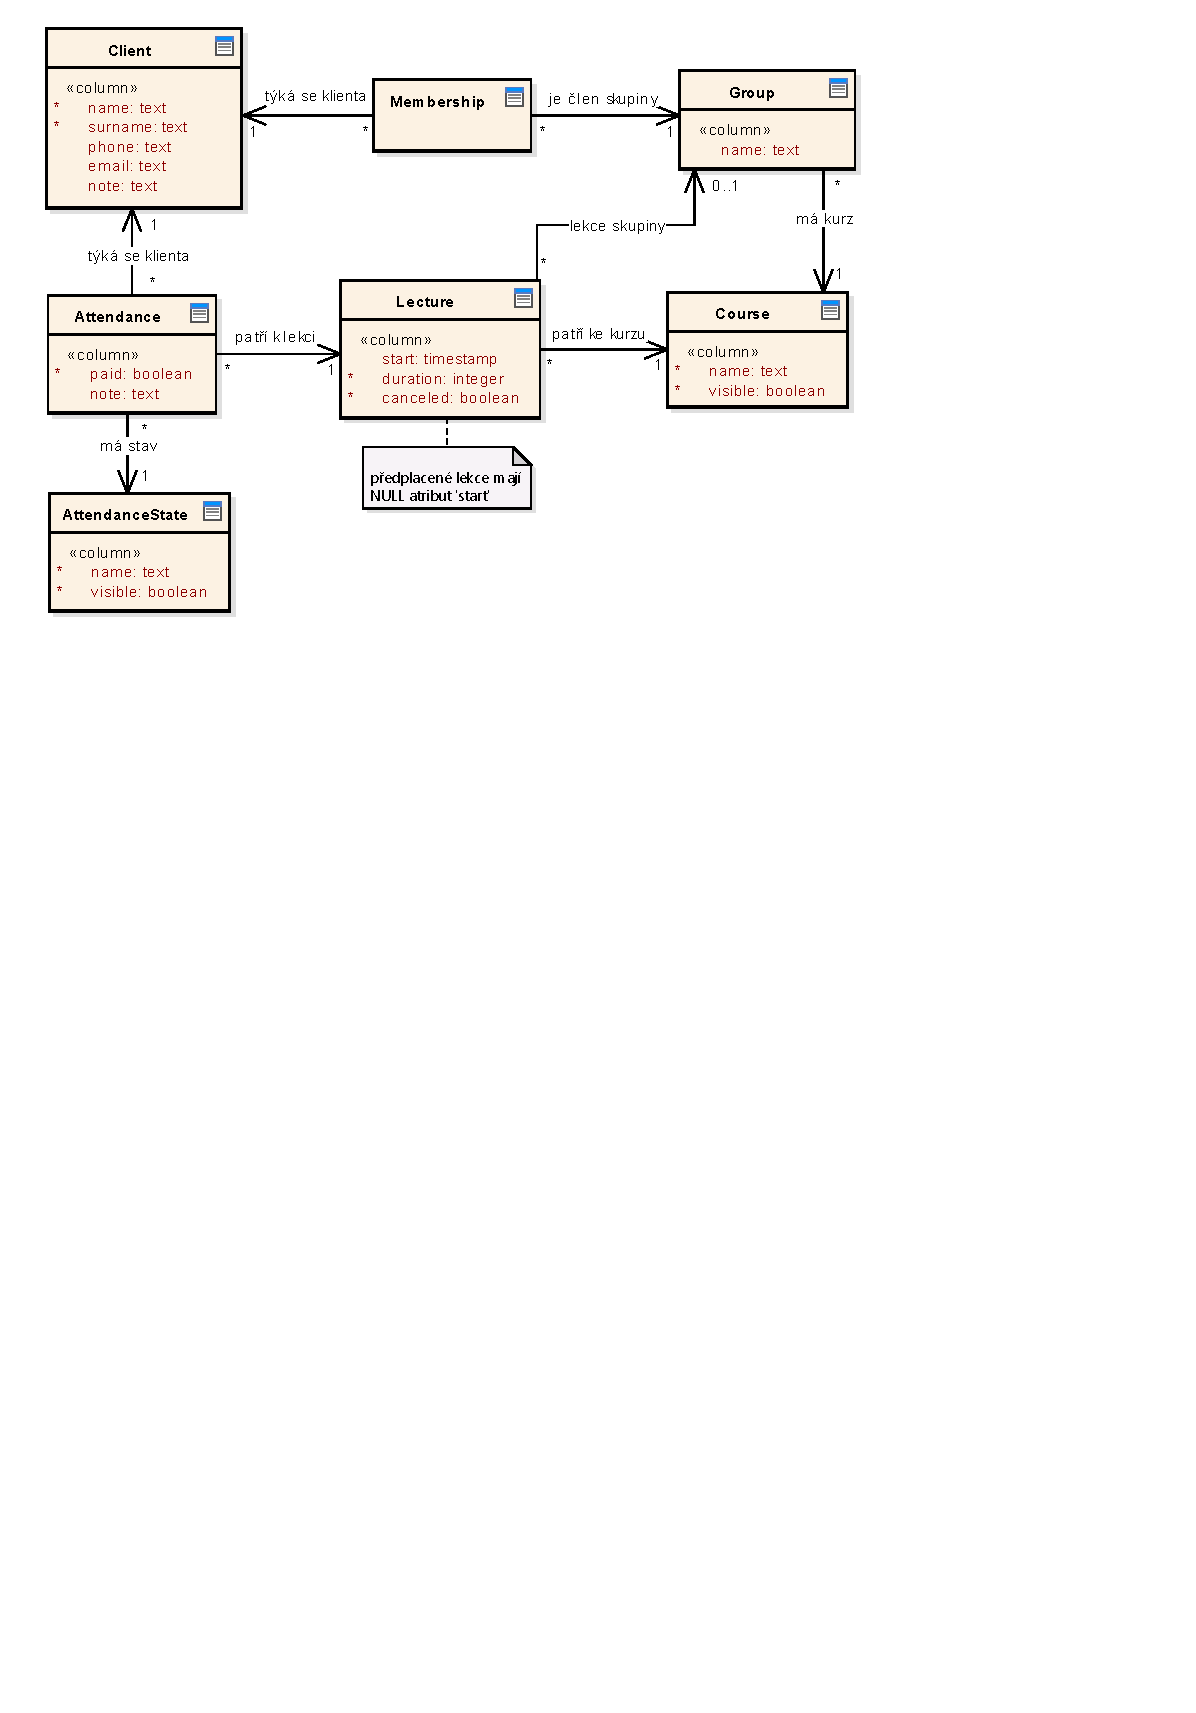
\includegraphics[width=1\textwidth]{img/db-model}
    	\caption[Logický datový model]{Logický datový model}\label{fig:db-model}
    \end{figure}
    
        \subsection{Client}
        Entita klienta slouží k evidenci informací o klientovi, vyžadováno je jméno a příjmení, nepovinně telefonní a e-mailový kontakt na rodiče a poznámka. Kontakty jsou nepovinně zejména kvůli tomu, že doteď nebyly evidovány na jednom místě a někdy dokonce vůbec a bude potřeba již stávající klienty do evidence samozřejmě přidat (viz. podsekce~\ref{subsec:klienti}).
        
        \subsection{Membership}
        Členství slouží ke dvěma účelům. Zaprvé k dekompozici M:N vztahu klienta a skupiny (klient může být ve více skupinách a skupiny mohou mít více klientů), vím tedy, který klient patří do které skupiny. Zadruhé pro možné budoucí využití (původní záměr byl vytvořit atributy pro začátek a konec členství, na základě další analýzy a návrhů se ukázalo, že ale zatím postačí jednodušší varianta, tedy zda je teď členem nebo není).
        
        \subsection{Group}
        Skupina slouží k evidenci jednotlivých skupin. Atribut jméno skupiny je nepovinný (ačkoliv bude obvykle používán, jeho použití není vyžadováno, protože to není nutné). Dále skupina ví, ke kterému kurzu náleží, tato vazba je zde proto, že skupiny už od počátku svého vytvoření patří vždy k právě jednomu kurzu (oproti klientovi, který takovou vazbu nepotřebuje) -- toho se využívá například při vytváření skupinové lekce, kdy se automaticky jako kurz zvolí kurz skupiny.
        
        \subsection{Course}
        Kurz drží dva atributy: jméno kurzu a viditelnost, oba jsou povinné. Viditelnost slouží k tomu, aby bylo v rámci aplikace možné při přidávání lekcí či skupiny skrýt z možností kurzu příslušný kurz, pokud už není provozován (aby byla zachována předchozí evidence lekcí daného kurzu).
        
        \subsection{AttendanceState}
        Stav účasti slouží k evidování možností stavu účasti klientů na kurzu, předpokládanými stavy jsou např. \enquote{omluven}, \enquote{neomluven} a \enquote{OK}. Drží dva atributy: název stavu účasti a viditelnost, oba jsou povinné. Viditelnost opět slouží k tomu, aby bylo v rámci aplikace možné pro nově přidávané lekce skrýt z možností stavu účasti klienta příslušný stav, pokud už není využívaný (aby byla zachována předchozí evidence lekcí daného kurzu). Tím, že mám jednu entitu, která říká, jaké jsou možné stavy účasti, může být aplikace konzistentní, zároveň pro úpravu názvu není potřeba upravit každý stav zvlášť, dále lze jednoduše stav účasti přidat a začít jej používat, případně jej přestat používat a skrýt z budoucích nabídek (nebo v případě žádného použití i smazat).
        
        \subsection{Attendance, Lecture}
        Vzhledem k úzkému propojení těchto dvou entit spojuji jejich popis do jedné podsekce. Účast a lekce jsou jádrem aplikace a vzhledem k tomu, že je k nim potřeba z různých entit přistupovat, věnoval jsem dostatečný čas jejich návrhu, aby byl kvalitní a nebylo nutné jej v průběhu vývoje zásadně měnit.
        
        Je potřeba evidovat lekce, každá má povinné atributy trvání (plánuje se funkcionalita upozornění na překryv lekcí), zda je zrušena (díky tomu lze jednoduše zrušit i skupinové lekce, oproti přístupu, kdy bych zrušení evidoval prostřednictvím entity stavu účasti) a nepovinnou časovou značku začátku lekce (tzv. timestamp). V případě, že se jedná o naplánovanou lekci bez zatím známého konkrétního termínu, atribut začátku obsahuje hodnotu \verb|null|. Ke každé lekci eviduji k ní náležící právě jeden kurz a nepovinně také skupinu, pokud se nejedná o individuální kurz. Tato vazba je potřeba pro individuální lekce (skupiny jsou řešeny vazbou přímo z entity skupin), tento způsob byl shledán po vyhledávání alternativních možností tím nejvhodnějším.
        
        Entita účasti je úmyslně oddělena od lekce, aby každý klient, kterého se lekce týká, mohl mít své údaje o účasti (což je v případě skupiny potřeba). Každá účast tedy ví, ke které jedné lekci a jednomu klientovi náleží, také je k ní navázán právě jeden stav účasti příslušného klienta.
        
        Příkladem budiž lekce z pohledu entity účasti -- pro případ individuální lekce má účast navázaného jednoho klienta, jeden stav účasti a jednu lekci, která je dále navázána na jeden kurz. Pro případ skupinové lekce se čtyřčlennou skupinou jsou využity 4 záznamy v klientech, jeden záznam ve skupině a tyto záznamy jsou spojeny entitou členství. Skupině náleží jeden kurz. Nyní mohu vytvořit pro každého z účastníků účast navázanou na každého z nich, na stav účasti a také všechny navázané na stejnou lekci.
        

    \section{Architektura}\label{architektura}
    Na obrázku~\ref{fig:deployment-diagram} je diagram nasazení. Architektura má tři části: server, klient a databázový server. Na klientovi (počítač, telefon, tablet) běží webový prohlížeč. Na serveru běží webový server \href{http://gunicorn.org/}{Gunicorn}, což je Python WSGI HTTP Server (WSGI znamená, že splňuje požadavky na rozhraní Web Server Gate Interface, tedy umožňuje komunikovat Django aplikaci, která WSGI vyžaduje, s webovým serverem). PostgreSQL databáze bude na samostatném serveru.
    
    \begin{figure}[ht]\centering
    	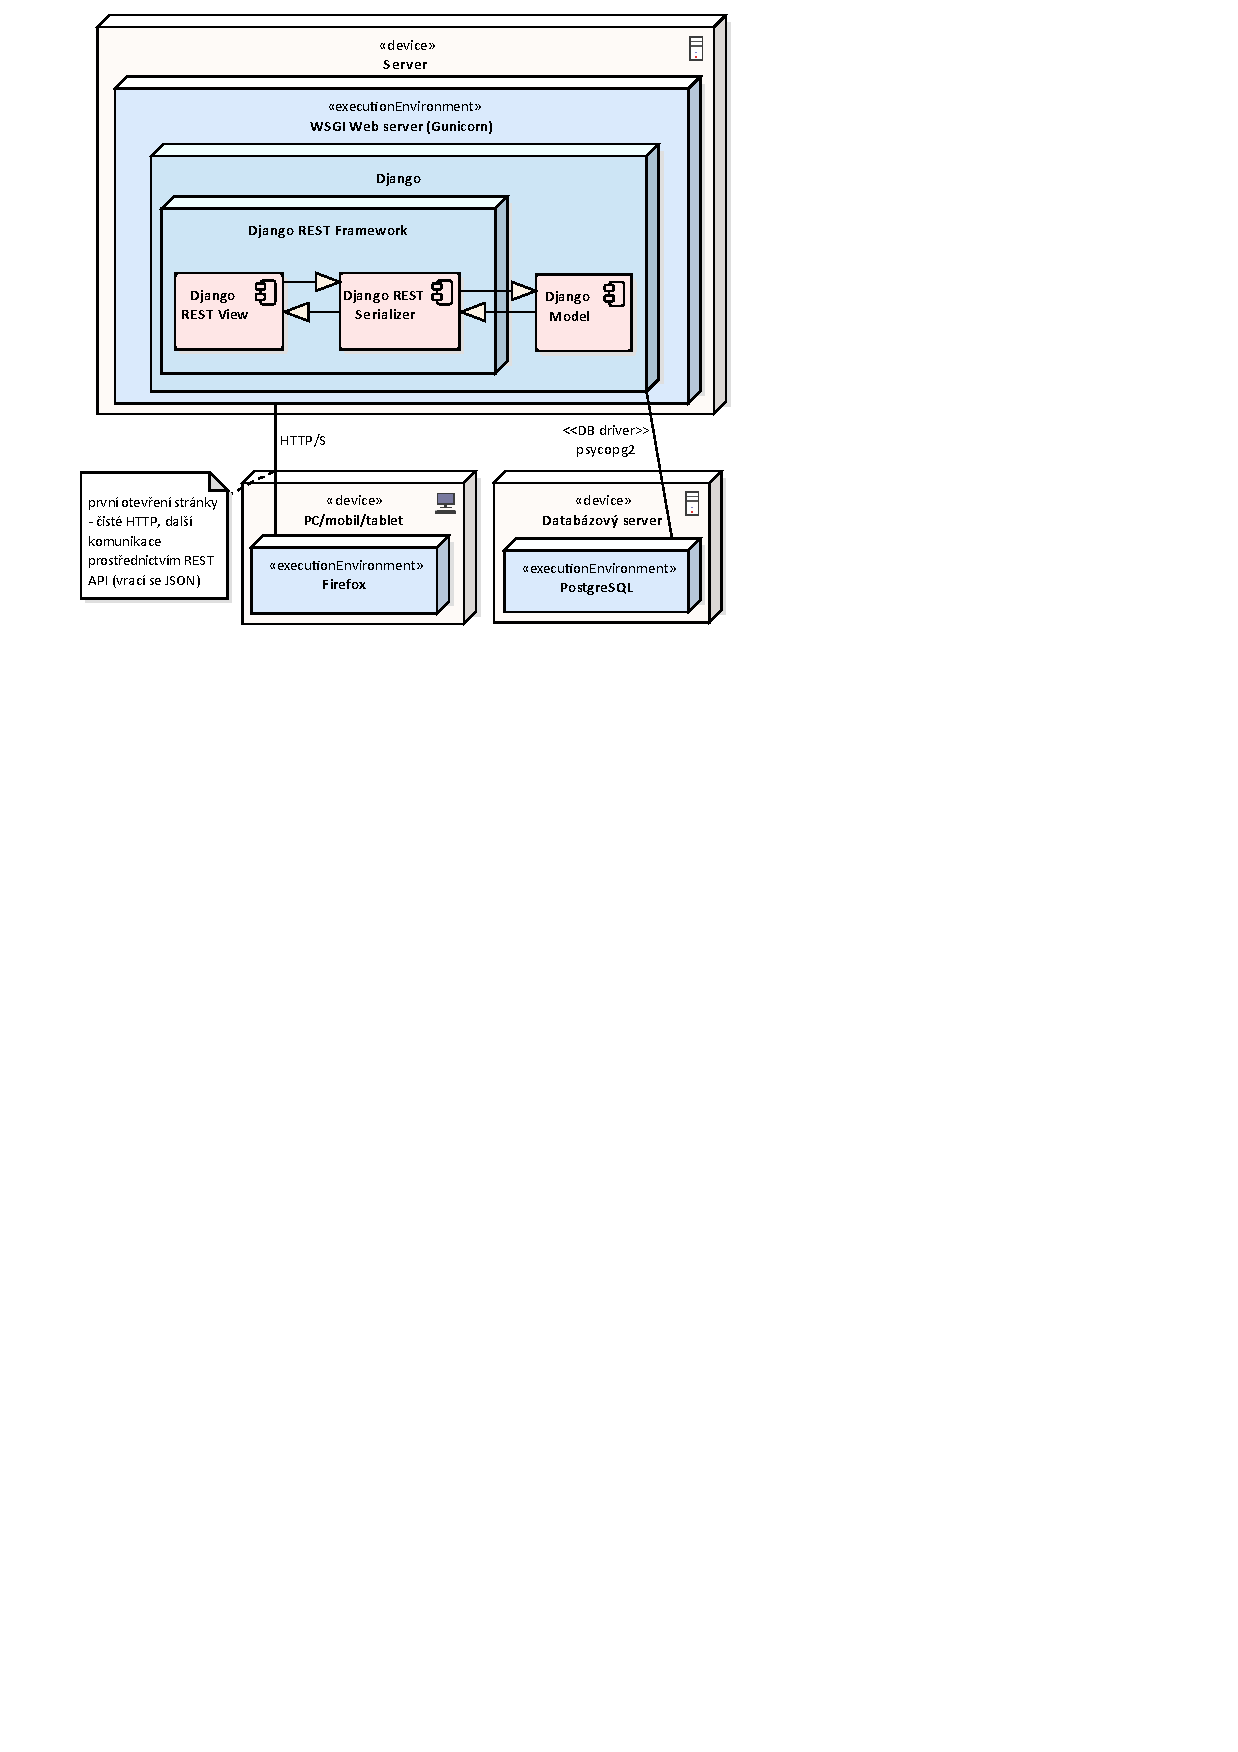
\includegraphics[width=1\textwidth]{img/deployment-diagram}
    	\caption[Diagram nasazení]{Diagram nasazení}\label{fig:deployment-diagram}
    \end{figure}
    
    Jak již bylo řečeno v sekci~\ref{reseni}, serverová část je v jazyce Python a frameworku Django. S klientskou částí, která je v jazyce Javascript a frameworku React, komunikuje serverová část přes REST API ve formátu JSON. Django je postavené na architektuře MVT (popis v sekci~\ref{mvc}) a React na architektuře CBA (popis v sekci~\ref{cba}). První požadavek a odpověď budou čistě v HTTP/S, tedy klient požádá o stránku, server mu ji celou vrátí, další komunikace už bude probíhat přímo přes REST API a odpovědi budou v JSON (díky tomu může být aplikace SPA, viz. podsekce~\ref{spampa}). Python, a tedy i Django, umí v základu komunikovat pouze s SQLite databází, pro další databáze je třeba využít adaptér -- pro PostgreSQL se používá psycopg2. O vyřízení API požadavků je požádán Django REST Framework, konkrétně část View, která poté prostřednictvím Serializeru využije příslušné Django Modely (tedy ORM) a z databáze tak získá data.
    
    \section{Uživatelské prostředí}
    Návrh uživatelského prostředí je neodmyslitelnou součástí tvorby webové aplikace. Vzhledem k tomu, že byl návrh tvořen v několika iteracích, zvolil jsem pohodlnější a rychlejší kreslení na papír. Díky tomu jsme při konverzaci nad budoucí podobou aplikace s lektorkou mohli některé nápady okamžitě zahodit a vytvořit bez problémů nové.
    
    \begin{figure}[ht]\centering
    	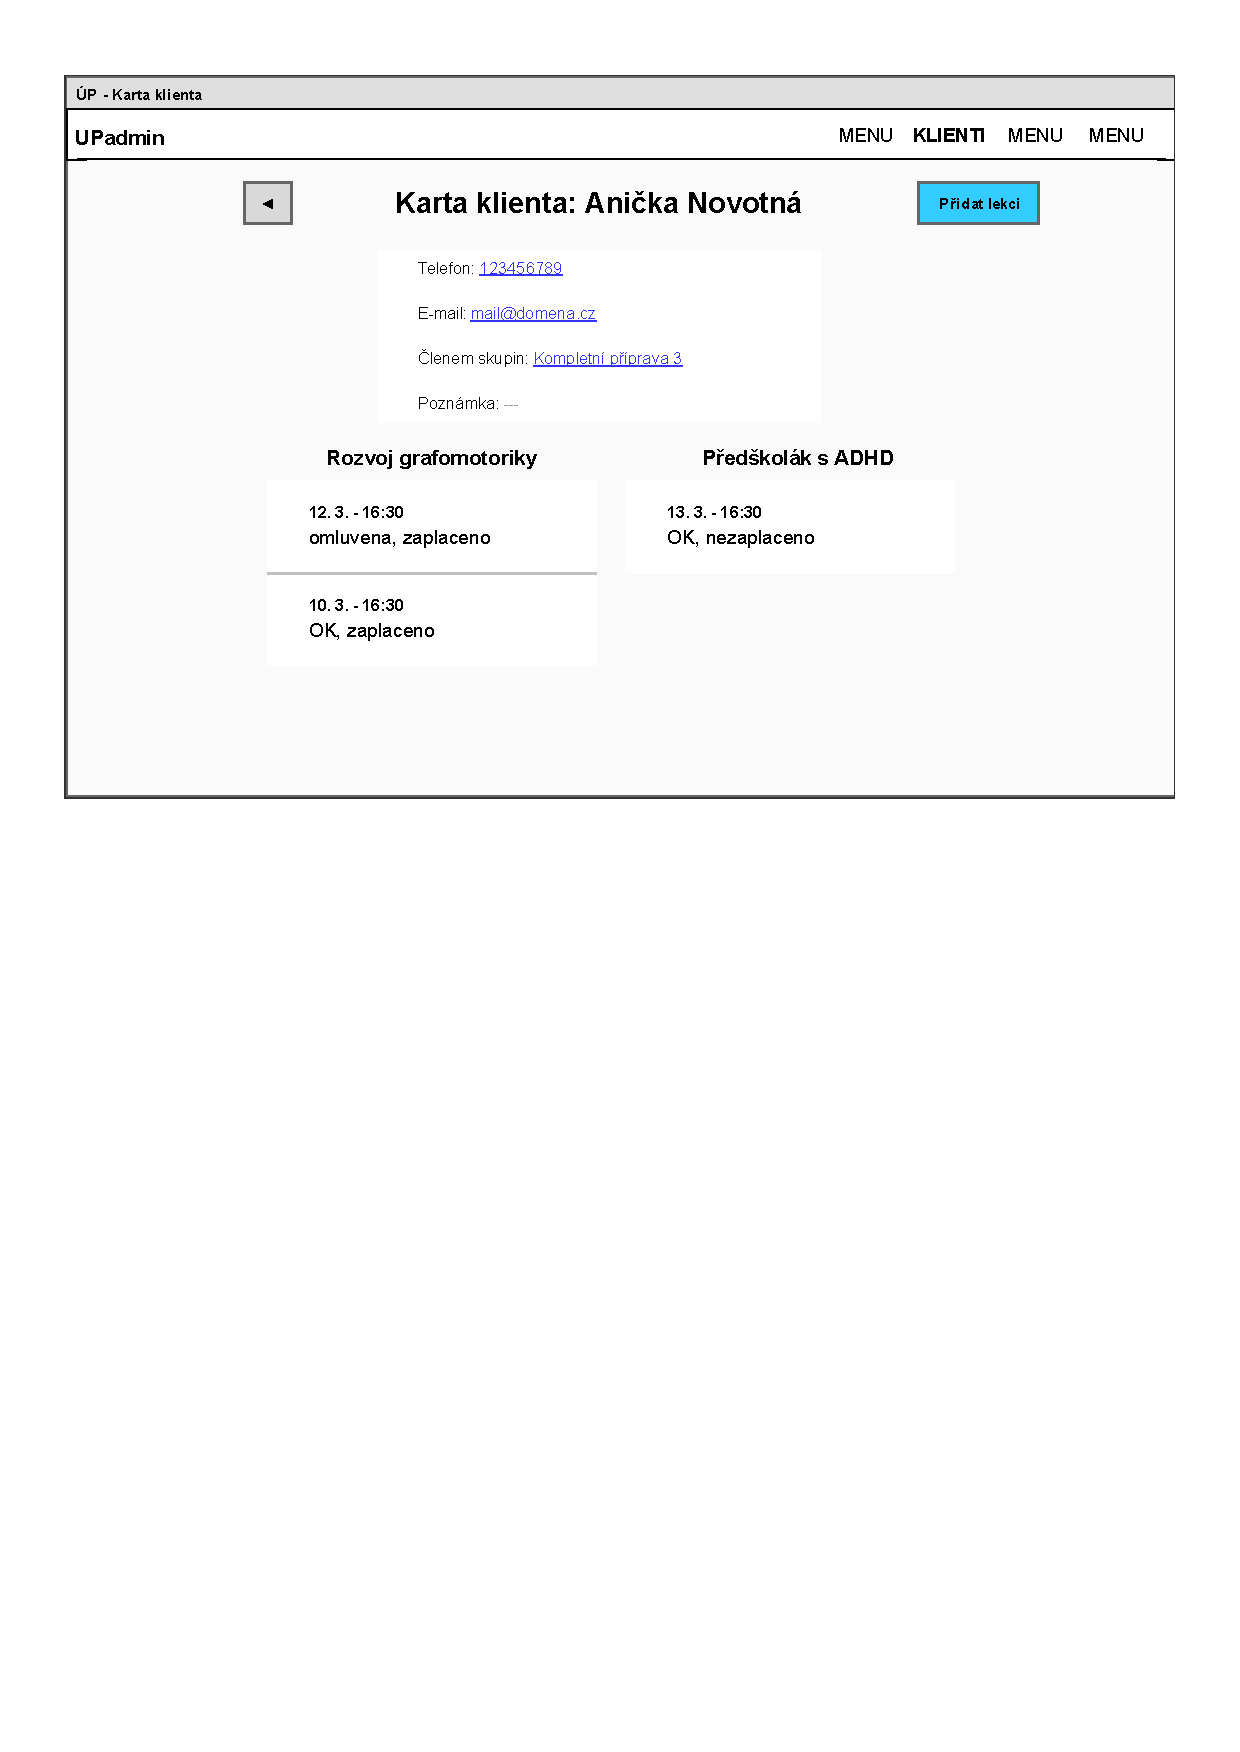
\includegraphics[width=1\textwidth]{img/ui-navrh}
    	\caption[Návrh karty klienta]{Návrh karty klienta}\label{fig:ui-navrh}
    \end{figure}
    
    Na obrázku~\ref{fig:ui-navrh} je jeden z návrhů z poslední iterace překreslený z papíru do aplikace \href{https://pencil.evolus.vn/}{Pencil}, jedná se o návrh karty klienta. Na základě těchto návrhů jsme doiterovali až do stavu, kdy jsme přesně věděli, co od aplikace čekat.
    
    \section{Komunikační rozhraní}
    Bylo potřeba navrhnout API tak, aby vystavilo všechny příslušné body potřebné pro práci na klientské části. Při návrhu jsem vycházel mj. z doporučení v~\cite{api-bestpractises} -- pro všechny body jsou názvy v množném čísle, využívám naplno všechno dostupné HTTP metody GET, POST, PUT, PATCH a DELETE, nevystavuji zbytečně adresy obsahující prováděné akce (např. vytvoření) a adresa všech níže dále uvedených bodů API vždy začíná \verb|/api/v1/| (obsahuje tedy i označení verze API).
    
    Jak bylo již řečeno v předchozím odstavci, API kromě běžných operací umožňuje také PATCH požadavek, ten slouží k datově méně náročné částečné aktualizaci údajů. Tuto metodu lze použít například v případě označení lekce jako zaplacené -- v tomto případě není nutné přenášet další údaje, stačí \verb|id| a upravovaný údaj. GET požadavky často, z důvodu snížení počtu požadavků na server, rovnou obsahují zanořená data (která jsou stejně vždy potřeba).
    
    \newcommand{\apiA}{0.33}
    \newcommand{\apiB}{0.14}
    \newcommand{\apiC}{0.43}
    
        \subsection{Klienti}
        Bod pro klienty pracuje s klíči \verb|id|, \verb|name|, \verb|surname|, \verb|phone|, \verb|email| a \verb|note|.
        Pro GET požadavky jsou klienti seřazeni vždy podle abecedy vzestupně, a to podle příjmení a poté jména.
        
            {\centering
            \begin{tabular}{p{\apiA\textwidth}p{\apiB\textwidth}p{\apiC\textwidth}}&&\\
                \verb|clients/|             & \textbf{GET}      & vrátí všechny klienty\\
                \verb|clients/|             & \textbf{POST}     & vytvoření nového klienta\\
                \verb|clients/:id/|         & \textbf{GET}      & vrátí klienta s \verb|id|\\
                \verb|clients/:id/|         & \textbf{PUT}      & úprava klienta s \verb|id|\\
                \verb|clients/:id/|         & \textbf{PATCH}    & částečná úprava klienta s \verb|id|\\
                \verb|clients/:id/|         & \textbf{DELETE}   & smazání klienta s \verb|id| (lze smazat pouze pokud nemá žádné lekce)\\
            \end{tabular}}
            
        \subsection{Lekce}
        Bod pro lekce pracuje s klíči \verb|id|, \verb|start|, \verb|group|, \verb|canceled| a \verb|duration|, to ale není vše. V případě skupinové lekce klíč \verb|group| obsahuje zanořené informace o skupině. Součástí odpovědi jsou i zanořené informace o kurzu (klíč \verb|course|) a jednotlivých účastech klientů (klíč \verb|attendances|), které obsahují platbu (klíč \verb|paid|), poznámku (klíč \verb|note|) a navíc také zanořené informace o každém z klientů (klíč \verb|client|), stavu účasti (klíč \verb|attendancestate|), vypočítané informace o číslu lekce v pořadí (klíč \verb|count|) a zda je potřeba připomenout příští platbu (klíč \verb|remind_pay|). Vypočítané informace jsou pouze v odpovědích a při požadavcích na úpravu či vytvoření se neuvádějí, dále zanořené informace kromě samotných účastí se zadávají pouze formou \verb|klíč_id| (tedy např. \verb|attendancestate_id|).
        
        Každý z dotazů na lekce lze doplnit také o parametr \verb|ordering=start|, resp. \verb|ordering=-start| pro seřazení výsledků dle atributu \verb|start| vzestupně, resp. sestupně (s posledními třemi dotazy, které již výsledky filtrují, lze toto řazení připojit přes operátor \verb|&|), výchozí řazení je sestupně (tedy od posledních lekcí k nejstarším). Kromě dotazu s uvedeným přesným datumem v parametru se vrací i zrušené lekce.
        
            {\centering
            \begin{tabular}{p{\apiA\textwidth} p{\apiB\textwidth} p{\apiC\textwidth}}&&\\
                \verb|lectures/|            & \textbf{GET}      & vrátí všechny lekce\\
                \verb|lectures/|            & \textbf{POST}     & vytvoří novou lekci\\
                \verb|lectures/:id/|        & \textbf{GET}      & vrátí lekci s \verb|id|\\
                \verb|lectures/:id/|        & \textbf{PUT}      & úprava lekce s \verb|id|\\
                \verb|lectures/:id/|        & \textbf{PATCH}    & částečná úprava lekce s \verb|id|\\
                \verb|lectures/:id/|        & \textbf{DELETE}   & smazání lekce s \verb|id|\\
                \verb|lectures/?group=:id|  & \textbf{GET}      & vrátí lekce skupiny s \verb|id|\\
                \verb|lectures/?client=:id| & \textbf{GET}      & vrátí lekce klienta s \verb|id| (jen individuální)\\
                \verb|lectures/?date=:date| & \textbf{GET}      & vrátí lekce (bez zrušených) konající se v zadaný datum \verb|date| (formát \verb|YYYY-mm-dd|)\\
            \end{tabular}}
        
        \subsection{Skupiny}
        Bod pro lekce pracuje s klíči \verb|id|, \verb|name| a dále se zanořenými informacemi o kurzu (klíč \verb|course|) a  členech skupiny (klíč \verb|memberships| obsahující zanořené informace o každém z klientů). Pro úpravy a vytváření se opět místo zanoření atributy zadávají pouze formou \verb|klíč_id|.
        
            {\centering
            \begin{tabular}{p{\apiA\textwidth} p{\apiB\textwidth} p{\apiC\textwidth}}&&\\
                \verb|groups/|              & \textbf{GET}      & vrátí všechny skupiny\\
                \verb|groups/|              & \textbf{POST}     & vytvoří novou skupinu\\
                \verb|groups/:id/|          & \textbf{GET}      & vrátí skupinu s \verb|id|\\
                \verb|groups/:id/|          & \textbf{PUT}      & úprava skupiny s \verb|id|\\
                \verb|groups/:id/|          & \textbf{PATCH}    & částečná úprava skupiny s \verb|id|\\
                \verb|groups/:id/|          & \textbf{DELETE}   & smazání skupiny s \verb|id|\\
                \verb|groups/?client=:id|   & \textbf{GET}      & vrátí skupiny klienta s \verb|id|\\
            \end{tabular}}
        
        \subsection{Kurzy}
        Bod pro kurzy pracuje s klíči \verb|id|, \verb|name| a \verb|visible|.
        
            {\centering
            \begin{tabular}{p{\apiA\textwidth} p{\apiB\textwidth} p{\apiC\textwidth}}&&\\
                \verb|courses/|             & \textbf{GET}      & vrátí všechny kurzy\\
                \verb|courses/|             & \textbf{POST}     & vytvoří nový kurz\\
                \verb|courses/:id/|         & \textbf{GET}      & vrátí kurz s \verb|id|\\
                \verb|courses/:id/|         & \textbf{PUT}      & úprava kurzu s \verb|id|\\
                \verb|courses/:id/|         & \textbf{PATCH}    & částečná úprava kurzu s \verb|id|\\
                \verb|courses/:id/|         & \textbf{DELETE}   & smazání kurzu s \verb|id| (lze smazat pouze pokud není přiřazený k žádné lekci nebo skupině)\\
            \end{tabular}}
            
        \subsection{Stavy účasti}
        Bod pro stavy účasti pracuje s klíči \verb|id|, \verb|name| a \verb|visible|.
        
            {\centering
            \begin{tabular}{p{\apiA\textwidth} p{\apiB\textwidth} p{\apiC\textwidth}}&&\\
                \verb|attendancestates/|    & \textbf{GET}      & vrátí všechny stavy účasti\\
                \verb|attendancestates/|    & \textbf{POST}     & vytvoří nový stav účasti\\
                \verb|attendancestates/:id/|& \textbf{GET}      & vrátí stav účasti s \verb|id|\\
                \verb|attendancestates/:id/|& \textbf{PUT}      & úprava stavu účasti s \verb|id|\\
                \verb|attendancestates/:id/|& \textbf{PATCH}    & částečná úprava stavu účasti s \verb|id|\\
                \verb|attendancestates/:id/|& \textbf{DELETE}   & smazání stavu účasti s \verb|id| (lze smazat pouze pokud není přiřazený k žádné účasti)\\
            \end{tabular}}
            
        \subsection{Účasti}
        Bod pro účasti je vytvořen pro snížení datové náročnosti běžné prováděných úprav. Pracuje s klíči \verb|id|, \verb|paid|, \verb|note|, \verb|attendancestate_id| a \verb|client_id|.
        
            {\centering
            \begin{tabular}{p{\apiA\textwidth} p{\apiB\textwidth} p{\apiC\textwidth}}&&\\
                \verb|attendances/:id/|     & \textbf{PUT}      & úprava účasti s \verb|id|\\
                \verb|attendances/:id/|     & \textbf{PATCH}    & částečná úprava účasti s \verb|id|\\
            \end{tabular}}
            
        \subsection{Přihlášení}
        Bod pro účasti pracuje s klíči \verb|username|, \verb|password| a \verb|token|.
        
            {\centering
            \begin{tabular}{p{\apiA\textwidth} p{\apiB\textwidth} p{\apiC\textwidth}}&&\\
                \verb|jwt-auth/|            & \textbf{POST}     & na základě zaslaných údajů uživatele vrátí token\\
                \verb|jwt-refresh/|         & \textbf{POST}     & na základě zaslaného (neexpirovaného) tokenu vrátí nový obnovený token\\
            \end{tabular}}
            
    
\chapter{Implementace}\label{implementace}
V této kapitole představím průběh samotné implementace. Je rozdělena do několika částí, nejprve popíši nástroje použité pro vývoj a přípravu prostředí. Poté se zaměřím na vytvoření základního nastavení serverové a klientské části, které bude výchozím krokem pro další sekce, v nichž postupně ukáži práci s datovou částí a tvorbu API. Tím připravím všechny součásti potřebné k fungování a vytvoření plnohodnotné klientské části v další sekci, uvedu zde také způsob komunikace se serverovou částí, tvorbu UI a další způsoby práce s JS a Reactem. Na závěr uvedu způsoby řešení bezpečnosti v aplikaci.

Nejproblematičtější fází se překvapivě stala konfigurace Djanga a Reactu tak, aby spolu tyto dvě části fungovaly, a také pokročilejší přizpůsobení API. Oběma problémům se budu také v této kapitole věnovat.

    \section{Nástroje pro vývoj}\label{nastrojeprovyvoj}
    Celá práce byla implementována ve vývojovém prostředí \href{https://www.jetbrains.com/pycharm/}{Pycharm Professional Edition} od Jetbrains na systému Windows 10, které nabízí nativní podporu pro všechny části tohoto projektu od samotného Pythonu (např. už ve výchozím nastavení podporuje virtuální prostředí pro izolaci jednotlivých prostředí pro různé projekty), Djanga až po React. Díky tomu lze využít funkce tohoto vývojového prostředí pro všechny používané jazyky a frameworky a také lze většina úkonů provádět pomocí grafického prostředí -- integrovaný terminál lze použít jen v případě, kdy je to opravdu potřeba. Dále existuje mnoho doplňků, které IDE rozšíří o podporu dalších funkcí, např. pro lepší práci s verzovacími nástroji a YAML formátem.
    
    Pro rychlejší vývoj, organizaci a také pro rozšíření znalostí a zkušeností jsem se rozhodl využít i další služby. Pro verzování využívám soukromý repozitář na \href{https://github.com/}{GitHubu}. Dále používám nástroj pro průběžnou integraci a nasazování \href{https://travis-ci.com/}{Travis CI}. Díky jednoduchému propojení s GitHubem se tak mohou samy spouštět při každém nahrání nové verze testy včetně těch pokročilejších a náročnějších a v případě úspěchu se aplikace nahraje na produkční server pro zákazníka. K tomu všemu slouží jediný soubor v kořenovém adresáři s názvem \verb|.travis.yml|, podrobněji příslušné části souboru popíši v kapitolách o testování~\ref{testovani} a nasazení~\ref{nasazeni}.
    
    \section{Příprava prostředí}
    Pro vývoj je potřeba nainstalovat další potřebné balíčky a závislosti, nejdříve jsem tedy nainstaloval do systému Python, jehož součástí je balíčkovací systém pip pro instalaci knihoven, a Node.js, jehož součástí je balíčkovací systém pro JS s názvem npm (Node.js je potřeba především pro vývoj, vytváření buildů a běh vývojového serveru, npm je vítaným ulehčením práce s knihovnami a závislostmi). V současnosti se často používá také balíčkovací systém yarn, který je ale třeba doinstalovat (například přes npm), jeho výhodou jsou stejné principy jako npm, ale mnohem vyšší efektivita a rychlost \cite{yarn}, pro tento projekt jej tedy z těchto důvodů používám. Pomocí těchto balíčkovacích systémů jsem dále nainstaloval poslední verze frameworku \href{https://www.djangoproject.com/}{Django} a nástroj \href{https://github.com/facebook/create-react-app}{create-react-app} pro jednoduché vytvoření React aplikace. Vzhledem k tomu, že vývoj bude probíhat v Pycharmu, není již potřeba dále řešit virtuální prostředí v Pythonu. Na závěr samozřejmě přidám a připravím v systému databázi PostgreSQL.
    
    \section{Základní nastavení serverové a klientské části}\label{zakladninastaveni}
    Začnu nejprve serverovou částí. V Djangu je potřeba nejprve vytvořit projekt a do něj poté přidávat jednotlivé komponenty, kterým se říká aplikace, projekt je tedy soubor aplikací a nastavení na jedné doméně. Pro vytvoření základní kostry projektu s výchozím nastavením jsem využil možností rozhraní Pycharmu, díky kterému stačí vyplnit základní informace o aplikaci a celou kostru připraví za mě, vytvořil jsem tedy projekt \verb|up|. Pro vytvoření aplikací jsem využil vestavěného manage.py terminálu v Pycharmu a v něm přes příkaz \verb|startapp| vytvořil dvě aplikace: \verb|admin| (pro samotnou aplikaci) a \verb|api| (pro API). Ty je poté potřeba v nastavení Djanga přidat do seznamu \verb|INSTALLED_APPS| v souboru s nastavením.
    
    \begin{listing}[ht]
    	\begin{minted}[bgcolor=bg]{python}
re_path(r'^', TemplateView.as_view(template_name="index.html"))
    	\end{minted}
    	\caption{Základní nastavení routování v urls.py}\label{lst:urls.py}
    \end{listing}
    
    Do serverové části zatím nebudu v této sekci příliš zasahovat, pro další práci ještě ale upravím aplikaci \verb|admin| tak, aby místo své výchozí stránky zobrazovala mou vlastní. Pro takto jednoduché zobrazení stačí využít již připravený generický pohled \verb|TemplateView| a jeho metodu \verb|as_view|, tedy do souboru \verb|urls.py| vložím kód~\ref{lst:urls.py}, který zařídí, že každému uživateli na jakékoliv adrese (kromě API, to nastavím až v sekci~\ref{sec:api}) ukážu daný soubor (zobrazení správné stránky v rámci webové aplikace bude zodpovědnost JS na klientské části).
    
    Serverová část je připravena, nyní popíši základní nastavení klientské části. Nástroj create-react-app umožňuje jednoduše vytvořit základní React aplikaci včetně všech základních nastavení a kostry. Takto jsem vytvořil aplikaci \verb|frontend|, tedy složku s tímto názvem, která obsahuje všechny potřebné součásti pro běh React aplikace. Součástí této připravené aplikace jsou mimo jiné tyto předkonfigurované součásti:
    \begin{itemize}
        \item transpiler Babel, který umožní používat bez obav JSX a další nové funkce z novějších ES standardů (viz. sekce~\ref{js}),
        \item bundlovací nástroj Webpack, který podle \cite{webpack-ackee} umožňuje:
            \begin{itemize}
                \item rozdělovat kód do modulů a napříč aplikací je importovat a znovupoužívat,
                \item spouštět server, který umožní rychlý vývoj díky \enquote{hot reloadingu} (tedy okamžité automatické projevení změn při úpravě kódu),
                \item automaticky spouštět transpilaci Babelem,
                \item po přeložení vytvořit ze všech modulů a částí kódu jeden či více balíčků, které pak lze jako běžné JS a další soubory (např. CSS) servírovat na produkci, kde už vývojový server neběží,
                \item s produkčními soubory provést další úpravy, například minifikaci (minimalizaci velikosti souboru) či označení hashem (aby prohlížeč poznal, zda může využít soubor z cache, nebo došlo ke změnám),
            \end{itemize}
        \item testovací nástroje a další knihovny umožňující rychlejší vývoj, vyšší kompatibilitu napříč prohlížeči, rychlejší načítání ad.
    \end{itemize}
    Všechny tyto součásti používám, včetně nových specifikací ECMAScript, JSX apod., díky všem nástrojům není důvod k obávám z nekompatibility a mohu z jejich použití pouze profitovat. Uvedené operace se soubory, které provádí Webpack a Babel by většinou šly provést až na produkci u uživatele, ale jednalo by se o zbytečně krkolomné a pomalé řešení, proto se provádí již při nahrávání na integrační/produkční server.
    
    Nyní tedy mám na lokálním počítači připravené Django a React, obě tyto části běží na svých vývojových serverech a na odlišných portech zobrazují své výchozí stránky. Je třeba tyto dvě části propojit. V případě lokálního prostředí musí spolupracovat tak, abych nepřišel o žádné výhody jako např. hot reloading a hash v názvu -- tedy aby nebylo při každé úpravě potřeba v Djangu měnit adresu souborů kvůli odlišné hodnotě hashe. V případě produkčního prostředí je třeba přizpůsobit konfiguraci tomu, že zde už poběží pouze jeden server (Gunicorn), na kterém bude Django. Tato část se vzhledem k mé dosavadní neznalosti těchto technologií ukázala jako poměrně náročná, protože bylo potřeba upravit kódy na obou stranách (tedy jak v Djangu, tak pro React v konfiguraci Webpacku) a ještě k tomu toto udělat prakticky dvakrát, jak pro lokální vývoj, tak pak odlišně pro produkci. Nakonec se mi ale podařilo tuto problematiku vyřešit, řešení vychází z článku \cite{webpack-loader2} a také staršího článku autora obou použitých knihoven \cite{webpack-loader1}, v následujícím odstavci jej stručně popíši.
    
    Díky nástroji create-react-app \cite{cra} mám k dispozici jednoduchou kostru, která mi ale neumožní hlubší zásahy do další konfigurace vnitřních součástí. Je tedy potřeba pomocí příkazu \verb|yarn eject| \enquote{vysunout} konfigurační soubory a závislosti tak, abych k nim měl přístup a mohl je upravit. Nyní potřebuji další dvě knihovny, každou pro jednu stranu -- do JS přidám knihovnu \href{https://github.com/owais/webpack-bundle-tracker}{webpack-bundle-tracker} (dále jen tracker), která vyextrahuje potřebné informace z Webpacku do JSON souboru \cite{webpack-bundle-tracker} (např. názvy vygenerovaných souborů) a do Djanga přidám knihovnu \href{https://github.com/owais/django-webpack-loader}{django-webpack-loader} (dále jen loader), která tyto informace bude konzumovat a umožní použít vygenerované soubory Webpackem v Djangu \cite{django-webpack-loader}. Tento JSON soubor bude tedy propojovat Webpack s Djangem.
    
    Když mám připravené tyto knihovny a kompletní kostru aplikace po vysunutí, je potřeba upravit konfiguraci Webpacku pro lokální i produkční prostředí tak, aby spolupracoval s trackerem a soubory byly tam, kde je bude očekávat loader, který konzumuje výstup trackeru (a aby totéž umožnil i pro lokální prostředí s hot reloadingem). Také je potřeba nakonfigurovat loader, to lze provést v souboru s nastavením Djanga, oproti původní vygenerované kostře Djangem budou ale soubory s nastavením dva -- jeden obecný, jehož součástí budou také informace pro lokální prostředí a jeden produkční, který bude obsahovat import předchozího a přetíží konfiguraci potřebných částí tou svojí (to se týká nejen této části, ale později například i různých nastavení databází pro různá prostředí). V těchto nastaveních jsem nakonfiguroval loader tak, aby konzumoval správný soubor ze správného místa a také jsem nastavil adresy statických souborů tak, aby je Django zahrnulo do shromažďování souborů prováděného příkazem \verb|collectstatic| (používá se při nasazení). Posledním krokem je vložení loaderem získaných souborů do webové stránky, aby se zobrazily uživateli, v tomto kroku tedy poprvé a naposledy v celé této práci použiji šablonovací systém Djanga (který by byl naopak hojně používaný v případě, že bych nezvolil SPA architekturu) -- do kostry výchozí stránky Djanga vložím tagy, které z loaderu umístí příslušné soubory do stránky (tedy JS a CSS). Zjednodušená verze této stránky, která zaručí zobrazení celé aplikace, je na ukázce~\ref{lst:html} -- React aplikace se vkládá do elementu \verb|root|. 
    
    Je hotovo, po provedení příkazu \verb|manage.py runserver| a \verb|yarn start| Django ukazuje webovou stránku, na které je zobrazena výchozí stránka Reactu, a to jak v lokálním prostředí, tak na produkci. 
    
    \begin{listing}[ht]
    	\begin{minted}[bgcolor=bg]{html}

<!DOCTYPE html>
<html lang="cs">
<head>
    <meta charset="UTF-8"/>
    <meta name="viewport" content="width=device-width,
                                   initial-scale=1,
                                   shrink-to-fit=no">
    <title>ÚPadmin</title>
</head>
<body>
<div id="root">
    <h2>Načítání...</h2>
</div>

</body>
</html>
    	\end{minted}
    	\caption{Základní stránka webové aplikace}\label{lst:html}
    \end{listing}
    
    \section{Datová část}\label{sec:datovaCast}
    K již nainstalovanému PostgreSQL jsem ještě nainstaloval vývojové prostředí pro databáze od Jetbrains s názvem DataGrip, díky kterému budu moci jednoduše nahlížet jak do lokální databáze, tak do databáze na produkčním serveru a případně provádět i další operace. Jak jsem již zmínil v sekci s návrhem architektury~\ref{architektura}, je potřeba použít adaptér \href{http://initd.org/psycopg/}{psycopg2}, ten umožní v Pythonu, a tedy i Djangu, používat databázi PostgreSQL. Do nastavení Djanga přidám tuto databázi a zbývá definovat tabulky v databázi.
    
    Při návrhu datového modelu v sekci~\ref{datovymodel} jsem nastínil, že díky frameworku mám výrazně ulehčenou práci s databází (a je třeba říci, že pokud člověk doteď žádný framework s touto funkcionalitou nepoužíval, je to opravdu obrovský krok kupředu), v Djangu není potřeba mít skripty pro vytvoření databáze, jediným zdrojem pravdy jsou Django modely definující jednotlivé entity, jejich atributy a chování. Následné další úpravy databáze na základě modelů se provádí prostřednictvím takzvaných migrací. V ukázce~\ref{lst:models} je jeden z modelů, konkrétně lekce, vybral jsem jej proto, že je na něm možné ukázat více věcí -- je zde vidět pět atributů, některé jsou nepovinné (\verb|start| a \verb|group|), reprezentují různé typy polí (kladné číslo, cizí klíč, boolean, časová značka) a u cizích klíčů je vidět, na který model odkazují, mohou mít přidělené jméno (použije se při využití opačného vztahu v modelu skupin) a také mají definované chování při smazání příslušného záznamu, tedy kurz se podaří smazat pouze když k němu nejsou žádné lekce (ošetření, aby se omylem nepřišlo o záznamy z historie) a v případě smazání skupiny se smažou mj. všechny její lekce.
    
    \begin{listing}[ht]
    	\begin{minted}[bgcolor=bg]{python}
class Lecture(models.Model):
    start = models.DateTimeField(null=True)
    canceled = models.BooleanField()
    duration = models.PositiveIntegerField()
    course = models.ForeignKey(Course, on_delete=models.PROTECT)
    group = models.ForeignKey(Group, related_name='lectures',
                              on_delete=models.CASCADE,
                              null=True)
    	\end{minted}
    	\caption{Ukázka modelu lekce ze souboru models.py}\label{lst:models}
    \end{listing}
    
    Postup při používání zmíněných migrací je jednoduchý. Při vytvoření či úpravě modelů je potřeba zavolat \verb|manage.py makemigrations| (vytvoří se soubor s migracemi na základě provedených úprav, v případě nejasností nebo potřebě dalších informací jsem vyzván k doplnění, tedy např. pokud měním atribut z nepovinného na povinný, jsem vyzván k zadání výchozí hodnoty, která bude doplněna do stávajících záznamů bez vyplněného atributu) a poté změny aplikovat \verb|manage.py migrate|. V praxi tedy při vývoji upravím model, vytvořím příslušným příkazem soubor s migracemi (a s tím související doplňující informace), zkontroluji správné výsledky, provedu migraci, zkontroluji funkčnost a výsledek zašlu do verzovacího systému, Travis a Heroku poté provedou příslušné migrace a změny jsou úspěšně provedeny ve všech prostředích konzistentně. Také je třeba dodat, že první migrací nevzniknou pouze mnou definované tabulky, ale také pomocné tabulky Djanga potřebné pro správný chod (např. tabulka s uživateli, provedenými migracemi ad.).
    
    \section{API}\label{sec:api}
    Mám připravený základ serverové části, tedy Djanga, které servíruje stránku s React aplikací, a také modely Djanga umožňující práci s entitami v projektu. Je potřeba vytvořit REST API, které umožní Reactu komunikovat se serverovou částí. V této části stručně shrnu, jak tvorba API probíhala. Vzhledem k tomu, že s tvorbou API je spojeno spoustu opakování podobného kódu, rozhodl jsem se využít služby dalšího frameworku, který mi v Djangu obstará jednoduché vytvoření REST API. Frameworků existuje několik, zvolil jsem nejpopulárnější \href{http://www.django-rest-framework.org/}{Django REST Framework} (dále DRF), který poskytuje užitečné nástroje a konstrukty k efektivní tvorbě API a zároveň obsahuje velkou škálu doplňkových knihoven od dalších členů komunity \cite{drf2}. Pro následné testování a úpravy API jsem používal nástroj \href{https://www.getpostman.com/}{Postman}.
    
    Obecně se tvorba API v DRF dělí na několik částí: views (pohledy), serializery a URL mapování. Nejprve je potřeba zvolit URL adresu pro API požadavky, tato adresa bude jako jediná mít zvláštní chování, ostatní adresy jsou obslouženy Reactem (viz. nastavení v sekci~\ref{zakladninastaveni}). Před řádek v ukázce kódu~\ref{lst:urls.py} vložím další řádek uvedený v ukázce~\ref{lst:urls.py2} (pokud bych jej vložil za, tak vzhledem k působnosti dříve vloženého kódu by převzal zodpovědnost za API React, což nechci). Nyní už stačí definovat konečné URL body API, kde určím, která adresa využije který pohled, k tomu slouží v DRF router, který umožní v souboru \verb|api/urls.py| jednoduchým způsobem definovat spojení URL adres s pohledy, v ukázce kódu~\ref{lst:apirouter} uvádím část pro lepší pochopení -- vybral jsem dva pohledy, které v dalším odstavci podrobněji ve zkratce představím a ukážu na nich další kroky při tvorbě API.
    
    \begin{listing}[ht]
    	\begin{minted}[bgcolor=bg]{python}
path('api/v1/', include('api.urls')),
    	\end{minted}
    	\caption{Nastavení routování pro API v souboru urls.py}\label{lst:urls.py2}
    \end{listing}
    
    \begin{listing}[ht]
    	\begin{minted}[bgcolor=bg]{python}
router = routers.DefaultRouter()
router.register('courses', views.CourseViewSet)
router.register('groups', views.GroupViewSet)
    	\end{minted}
    	\caption{Ukázka routeru pro API v souboru api/urls.py}\label{lst:apirouter}
    \end{listing}
    
    DRF nabízí několik možností, jak vyřešit pohledy. Zvolil jsem tu, která by měla umožnit velmi jednoduše definovat celé API a obstarat automaticky pohled jak na detail (instanci entity), tak na kolekci (všechny instance entity) včetně všech operací, nazývá se ViewSet a API pohledy úzce mapuje na Django modely. Pohled může být definován poměrně snadno, jak je vidět v ukázce kódu~\ref{lst:apiview1} ze souboru \verb|api/views.py| -- vytvořil jsem pohled pro kurzy, definoval jsem \verb|queryset|, tedy dotaz, který získá obsah pro odpověď na požadavek na API (v tomto případě i seřazený podle jména, to je definováno v modelu) a \verb|serializer_class|, tedy třídu použitou pro serializaci, validaci a deserializaci dat. Serializeru se budu věnovat v dalším odstavci. Ve druhé ukázce kódu~\ref{lst:apiview2} je vidět, že přetěžuji metodu \verb|get_queryset|, to mi umožní vrátit v API odpovědi vyfiltrované výsledky, v tomto případě vrátím buď všechny skupiny (seřazené podle jména, to je definováno v modelu), nebo v případě zadání \verb|id| klienta všechny skupiny (opět seřazené podle jména), ve kterých je členem. Pro pokročilejší filtrování v API a také umožnění řazení přes parametry v adrese je pak u některých dalších pohledů využita knihovna django-filter, po konfiguraci pouze stačí v API pohledech zadat příslušné povolené atributy pro filtrování.
    
    \begin{listing}[ht]
    	\begin{minted}[bgcolor=bg]{python}
class CourseViewSet(viewsets.ModelViewSet):
    queryset = Course.objects.all()
    serializer_class = CourseSerializer
    	\end{minted}
    	\caption{Jednoduchý pohled pro API v souboru api/views.py}\label{lst:apiview1}
    \end{listing}
    
    \begin{listing}[ht]
    	\begin{minted}[bgcolor=bg]{python}
class GroupViewSet(viewsets.ModelViewSet):
    serializer_class = GroupSerializer
    def get_queryset(self):
        qs = Group.objects.all() # qs znaci queryset
        id_client = self.request.query_params.get('client')
        if id_client is not None:
            qs = qs.filter(memberships__client=id_client)
        return qs
    	\end{minted}
    	\caption{Pokročilejší pohled pro API v souboru api/views.py}\label{lst:apiview2}
    \end{listing}
    
    Poslední chybějící součástkou, kterou jsem ještě neukázal, jsou serializery. V ukázkách kódu~\ref{lst:apiview1} a \ref{lst:apiview2} je vidět jejich používání, o kterém jsem mluvil v předchozím odstavci. Vzhledem k délce jejich kódu je na ukázce~\ref{lst:apiserializer1} vidět nejjednodušší serializer pro kurzy. K implementaci jsem použil \verb|ModelSerializer|, díky kterému je serializer úzce navázán na model a není potřeba opakovat zbytečně kód. Nevýhodou DRF je, že neposkytuje jednoduchou možnost práce s vnořenými zdroji, se kterými jsem v rámci návrhu počítal -- cílem bylo např. získat lekci spolu s údaji klienta, ale při úpravě lekce už údaje klienta nevyžadovat, pouze jeho \verb|id|. Dokumentace tohoto frameworku je sice poměrně rozsáhlá, ale často je také poměrně krkolomná a spoustu potřebných údajů je těžké nebo i nemožné dohledat. Nakonec jsem přišel na způsob, jak by se tento problém měl řešit, v příslušných serializerech bylo potřeba u dotyčných atributů vždy vytvořit dvojici atributů, kdy ten s údaji klienta bude pouze pro čtení a název bude totožný s modelem a druhý atribut bude mít odlišný název (zvolil jsem vždy přidání \verb|_id| k původnímu názvu) a bude určen pouze pro zápis (navíc je se strany DRF pro korektní fungování vyžadován argument \verb|queryset|, také je použit argument \verb|source|, aby se daný atribut choval jako atribut původní), lze vidět na ukázce~\ref{lst:apiserializer2}. 
    
    \begin{listing}[ht]
    	\begin{minted}[bgcolor=bg]{python}
class CourseSerializer(serializers.ModelSerializer):
    class Meta:
        model = Course
        fields = '__all__'
    	\end{minted}
    	\caption{Jednoduchý serializer pro API v souboru api/serializers.py}\label{lst:apiserializer1}
    \end{listing}
    
    \begin{listing}[ht]
    	\begin{minted}[bgcolor=bg]{python}
client = ClientSerializer(read_only=True)
client_id = serializers.PrimaryKeyRelatedField(
        queryset=Client.objects.all(), source='client',
        write_only=True)
    	\end{minted}
    	\caption{Práce se vnořenými zdroji v serializeru}\label{lst:apiserializer2}
    \end{listing}
    
    Druhým souvisejícím problémem, který jsem musel vyřešit, byla práce se vnořenými zdroji při požadavcích POST, PUT a PATCH, například při vytvoření lekce je potřeba vytvořit také pro každého člena účast apod. Nakonec i tento problém se mi podařilo vyřešit, konkrétně přetížením metod \verb|create| a \verb|update| v příslušných serializerech (ukázku neuvádím kvůli delším kódům). Vytvoření funkčního API především kvůli těmto dvěma zmíněným problémům trvalo mnohem déle, než jsem očekával.
    
    Součástí některých odpovědí API, například při GET požadavku na lekce, jsou další informace určené pouze pro čtení a vypočítané na základě dat v databázi, jsou jimi například informace o číslu lekce v pořadí (v rámci jednoho klienta a daného kurzu) či informace, zda má klient příště platit. Bylo tedy potřeba je důkladně promyslet a otestovat, příkladem budiž číslo lekce -- abych zjistil počet uběhlých lekcí, a tedy s přičtením jedné i pořadové číslo aktuální lekce, je potřeba vzít v úvahu, zda se jedná o naplánovanou lekci bez datumu (ta nemá číslo), o skupinovou lekci (zde se zjišťuje číslo jednodušeji, stačí vzít lekce skupiny, vyselektovat pouze ty, které jsou dříve než datum aktuální lekce, nejsou nenaplánované a ani zrušené) a nebo o individuální lekci (zde vezmu lekce klienta náležící k danému kurzu, pouze individuální, s určeným datumem, který je dříve než datum u aktuální lekce, nezrušené a se stavem účasti odpovídajícím tomu, že se dostavil).
    
    \section{Klientská část}
    Pro klientskou část je, jak jsem již zmínil při volbě architektury v sekci~\ref{reseni}, zvolena knihovna React, která mi umožní vytvořit interaktivní aplikaci a jednoduše ji dále rozšiřovat a rozvíjet díky architektuře CBA (viz. sekce~\ref{cba}). V této části stručně popíši, jak jsem při tvorbě klientské části postupoval.
    
    \subsection{Vzhled}
    Součástí tvorby klientské části bylo rozhodnutí, zda zvolit pro řešení UI nějakou předpřipravenou šablonu nebo framework. Co se týče šablon, nalezl jsem několik takových, které byly postaveny na Reactu, jako např. \href{https://github.com/MacKentoch/react-director-admin-template}{react-director-admin-template}, \href{https://github.com/booleanhunter/ReactJS-AdminLTE}{ReactJS-AdminLTE},
    \href{https://github.com/marmelab/admin-on-rest}{admin-on-rest} (který umožňuje napojit administraci přímo na REST API),
    \href{https://github.com/ant-design/ant-design-pro/}{Ant Design Pro},
    \href{https://github.com/mrholek/CoreUI-React}{CoreUI-React}, k jejich použití jsem ale nepřistoupil, protože by buď zbytečně ztížily orientaci v rámci aplikace, nebo měly špatnou (či čínskou) dokumentaci, omezené funkce zdarma apod. Také by se mohly hůře přizpůsobovat pozdějším požadavkům na změny UI.
    
    Rozhodl jsem se využít služby frameworku \href{https://getbootstrap.com}{Bootstrap}, který v lednu 2018 přišel s dlouho očekávanou přepracovanou 4.~verzí. Díky němu se mohu při vývoji mnohem hlouběji zaměřit na funkcionalitu, protože se postará o spoustu věcí za mě, dalším důvodem použití je také jeho popularita a rozšířenost \cite{bootstrap} mezi vývojáři. S Bootstrapem jsem nikdy nepracoval (volil jsem vždy svůj vlastní kód) a zaujaly mě novinky v poslední verzi, které by vývoj této aplikace usnadnily. Abych mohl Bootstrap pohodlně v Reactu používat, použil jsem nástroj \href{https://github.com/reactstrap/reactstrap}{reactstrap}, díky kterému mohu Bootstrap komponenty vkládat jako bezstavové komponenty Reactu.
    
    Pro pokročilejší úpravy jsem také použil knihovny \href{https://github.com/fkhadra/react-toastify}{react-toastify} pro oznámení, \href{https://github.com/JedWatson/react-select}{react-select} pro usnadnění tvorby a práce s poli ve formuláři, kde je potřeba provést intuitivní násobný výběr (např. členové skupiny). Napříč celou aplikací také používám balíček a nástroj pro ikony \href{https://fontawesome.com/}{Fontawesome} -- použiji zde poprvé nejnovější verzi 5, která je zcela přepracovaná a rozšířená oproti předchozím verzím, se kterými mám výborné zkušenosti (balíček bude v mnou zakoupené placené verzi se stylem ikon \enquote{solid}) a opět pro jednodušší použití jako komponenty Reactu použiji oficiální knihovnu \href{https://github.com/FortAwesome/react-fontawesome}{react-fontawesome}.
    
    \subsection{Základní práce s Reactem}\label{sec:zakladniPraceSReactem}
    Prošel jsem všechny potřebné závislosti, nástroje, knihovny a konfigurace a nyní tak mohu ukázat, jak jsem postupoval při samotné tvorbě aplikace v Reactu. Vývoj probíhal v nejnovější verzi 16.2, předem bych ale rád podotkl, že na závěr vývoje došlo k vydání verze 16.3, která přinesla několik novinek, zejména v oblasti životního cyklu komponenty (změna API) a Context API, které usnadňuje předávání dat mezi komponentami napříč jejich stromem \cite{react-blog1}. U Contextu bych se rád zastavil, teprve se začíná používat (byl představen na konci března 2018), ale už teď lze říci, že doplňuje chybějící článek Reactu, kvůli kterému mnoho vývojářů používalo Redux. Redux se používá se pro správu stavu aplikace, jak ale říká jeho autor a dnes také přední vývojář Reactu v \cite{react-blog3}, často se používá zbytečně a komplikuje tak vývoj aplikace, který by byl jinak mnohem rychlejší a kratší. Rozhodl jsem se pro tuto práci respektovat jeho doporučení, tedy nejdříve vytvořit čistou aplikaci v Reactu, pochopit všechny aspekty takové tvorby a fungování a pak teprve uvažovat o tom, zda je potřeba Redux využít (případně použít nové Context API). Aplikace nyní běží na verzi 16.3, zatím ale nevyužívá žádné z jejích novinek, vzhledem k úpravě API životního cyklu komponenty je ale potřeba počítat s drobnějšími změnami, které budu muset provést při vydání a přechodu na verzi~17 \cite{react-blog2}.
    
    Ještě než se pustím do popisu práce s Reactem, rád bych uvedl jednu z knih -- \textit{React Design Patterns and Best Practices} \cite{react-kniha}, ze které jsem při seznamování se s Reactem vycházel. Kromě podrobných popisů fungování jednotlivých součástí Reactu obsahuje mnoho rad a tipů, jak psát efektivní, rozšiřitelný, znovupoužitelný a čistý kód v Reactu. Vzhledem k její rozsáhlosti a pokročilosti s ní plánuji pracovat i při dalším vývoji této aplikace po odevzdání práce.
    
    V Reactu je vše rozdělené do komponent, které obsahují všechny závislosti, kódy a logiku -- obstarávají tak své korektní vykreslení a práci. Každá takováto komponenta může mít v sobě dva typy dat \cite{react-docs1}:
    \begin{itemize}
        \item \enquote{props} atributy, které může získat od rodiče, komponenta je nemůže měnit (patří do správy nadřazené komponenty), jsou tedy podobné parametrům funkcí,
        \item \enquote{state}, tedy stav, který se nedědí a je spravován uvnitř komponenty, je tedy podobný proměnným ve funkcích.
    \end{itemize}
    
    Díky těmto atributům React zařídí překreslení pouze té části stránky, kde nastala změna. Velmi jednoduchá bezstavová komponenta využívající nejnovější prvky syntaxe JS používaná napříč aplikací k informování, zda má klient příště platit, je v ukázce~\ref{lst:react1}. V aplikaci dále používám i pokročilejší stavové komponenty, pro lepší pochopení vkládám ukázku~\ref{lst:react2} obsahující komentáře s vysvětlením. Zdůrazním zde metodu \verb|componentWillReceiveProps|, která je zde proto, že v rodiči se provádí asynchronní požadavek na API a některý z jeho výsledků se předává do této komponenty, tedy do potomka, kde se na jeho základě komponenta překresluje. Vzhledem k tomu, že jsou \enquote{props} samy o sobě neměnné, je třeba nový stav z potomka zpracovat v této metodě a změny zde projevit do vlastního stavu komponenty.
    
    \begin{listing}
    	\begin{minted}[bgcolor=bg]{js}
import React from 'react'
import {Badge} from 'reactstrap'
const RemindPay = ({remind_pay}) =>
    (remind_pay && 
        <Badge color="warning" pill>Příště platit</Badge>)
export default RemindPay
    	\end{minted}
    	\caption{Jednoduchá bezstavová komponenta Reactu}\label{lst:react1}
    \end{listing}
    
    \begin{listing}[ht]
    	\begin{minted}[bgcolor=bg]{js}
import React, {Component} from "react"
// import dalších JS komponent a CSS souborů
export default class NazevKomponenty extends Component {
    constructor(props) {
        // nastavení stavu a dalších proměnných/props
    }
    dalsiFunkce = () => {
        // tělo funkce
    }
    componentDidMount() {
        // požadavky na API
    }
    componentWillReceiveProps(nextProps) {
        // aktualizace stavu při změně stavu rodiče
    }
    render() {
        // příprava dalších komponent a proměnných
        return (
            <div>{/* vykreslení v JSX */}</div>)
    }
}
    	\end{minted}
    	\caption{Kostra pokročilejší komponenty v Reactu}\label{lst:react2}
    \end{listing}
    
    \subsection{Routování a HTTP požadavky v Reactu}\label{subsec:reactPozadavky}
    Nyní chybí dořešit poslední dvě části v Reactu: routování a komunikaci přes API, ani jedno totiž React, jak již bylo řečeno v podsekci~\ref{react}, v základu neumí. Pro routování jsem zvolil knihovnu \href{https://reacttraining.com/}{React Router}, která mi umožní v Reactu snadno implementovat SPA a zajistí také fungování tak, jak by uživatel očekával, tedy při přechodech se mění URL adresa v prohlížeči, korektně funguje navigace napříč historií apod. K tomu využívám \verb|BrowserRouter|, který se nově objevil v přepracované poslední čtvrté verzi této knihovny. Ten totiž oproti staršímu \verb|HashRouter| využívá nativní HTML5 API pro historii (místo práce s fragmentem URL přidaným za znakem \verb|#|). Nutnou podmínkou pro jeho funkčnost je korektní a funkční routování i na straně serveru, to je díky kódu~\ref{lst:urls.py} zařízeno -- nic tedy nebrání v použití této novější komponenty.
    
    \begin{listing}[ht]
    	\begin{minted}[bgcolor=bg]{js}
getClients = () => {
    ClientService
        .getAll()
        .then((response) => {
            this.setState({clients: response, loading: false})
        })}
    	\end{minted}
    	\caption{Příklad funkce obstarávající požadavek na REST API}\label{lst:react3}
    \end{listing}
    
    Pro komunikaci Reactu s vystaveným REST API jsem použil velmi populární a častou volbu vývojářů nejen pro React, knihovnu \href{https://github.com/axios/axios}{Axios}. Ačkoliv se už pomalu začíná rozšiřovat standardizované JS Fetch API, Axios nabízí širší a jednodušší možnosti práce s asynchronními požadavky, např. odchytávání pomocí \enquote{interceptorů}, zabudovanou CSRF ochranu (viz. sekce~\ref{sec:bezpecnost}) a také zaručuje kompatibilitu ve všech prohlížečích \cite{axios}. Protože bylo potřeba mít k dispozici jednotnou správu nad všemi požadavky včetně odchytávání chyb a konfigurace, vytvořil jsem jednotné rozhraní pro požadavky, které jsem doplnil o vytvoření služeb pro každou využívanou část API. V samotné stránce, kde probíhá požadavek na API, tedy nejsou žádné konfigurační informace (ani URL adresa) a vše tak lze snadno upravit, případně i nahradit knihovnu pro požadavky. 
    
    Na ukázce~\ref{lst:react3} přikládám výsledný kód používající importovanou službu, která poté zavolá jednotné rozhraní pro požadavky -- tam teprve proběhne vytvoření a zaslání požadavku prostřednictvím Axiosu na API a v případě úspěchu se výsledek uloží do stavu komponenty a komponenta se tak překreslí. V této ukázce je také vidět přenastavení atributu \verb|loading|, díky tomu může být v příslušné komponentě zobrazena načítací animace, dokud komponenta neobdrží příslušná data. Tedy například při načítání lekcí v týdenním přehledu jsou okamžitě zobrazeny všechny pracovní dny i s jejich boxy, díky rozdělení na komponenty má každý box své načítání a tato animace zmizí vždy právě tehdy, když se načtou data do příslušného boxu. Uživatel mezitím může provádět další operace a vidí, kdy je požadavek dokončený.
    
    \subsection{Další práce s JS}
    Ačkoliv Babel spolu s dalšími polyfilly umožní vytvářet kód s co nejvyšší možnou kompatibilitou napříč různými prohlížeči, bylo třeba i tak dbát na její ověření. V rámci vývoje jsem například zjistil, že prohlížeče Safari a Internet Explorer pracují odlišně s datumy dle standardu ISO, což vyústilo v několik chyb v aplikaci (nezobrazení datumů ad.). Musel jsem tedy upravit práci s datumy tak, aby byl kód kompatibilní i v těchto prohlížečích. Další s ISO standardem související problém byl, že v JS se pracuje s datumy v tomto formátu pouze s časovou zónou UTC, ačkoliv jsou třeba v jiné. To vyústilo v situaci, že vždy mezi půlnocí a jednou hodinou ranní byly v týdenním přehledu zobrazeny špatné dny (tedy při letním čase dokonce od půlnoci do dvou hodin ráno), byl jsem tedy nucen pro tuto práci s datumy vytvořit vlastní funkce, které respektovaly i jiné časové zóny.
    
    \section{Bezpečnost}\label{sec:bezpecnost}
    Vzhledem k tomu, že se v aplikaci nacházejí důvěrné informace, je potřeba zvolit adekvátní úroveň zabezpečení. V této sekci stručně shrnu kroky, které jsem učinil k zabezpečení aplikace, zejména v oblasti zabezpečení komunikace a přihlášení.
    
    \subsection{Ochrana proti útokům}\label{sec:bezpecnostOchrana}
    Je potřeba využívat protokol HTTPS, díky kterému bude komunikace šifrovaná -- Heroku má pro aplikace bez vlastní domény zdarma SSL certifikát, bylo tedy nutné jen zajistit přesměrování veškeré komunikace na zabezpečenou variantu. To zajistí v konfiguraci Djanga nastavení proměnné \verb|SECURE_SSL_REDIRECT|.
    
    Ve webových aplikacích se často objevují některé bezpečnostní chyby, podle \cite{bezpecnost1} a \cite{bezpecnost2} zejména:
    \begin{itemize}
        \item \textbf{SQL Injection:} narušení SQL dotazu z důvodu špatného ošetření parametrů při tvorbě SQL dotazů,
        \item \textbf{XSS (Cross-Site Scripting):} vložení škodlivého kódu kvůli nedostatečnému ošetření vstupů od uživatele,
        \item \textbf{CSRF (Cross-Site Request Forgery):} tajné vykonání požadavku z důvodu neošetření původu požadavku,
        \item \textbf{Clickjacking:} součástí podvodné stránky je jiná stránka a uživatelem provedená akce vyústí v nezamýšlené akce na jiné stránce.
    \end{itemize}
    
    Využil jsem možnosti Djanga v oblasti bezpečnosti \cite{bezpecnost1} a nakonfiguroval jej tak, aby rizika hrozeb eliminovalo na minimum. Díky ORM není problém s SQL Injection a díky dalším konfiguracím ani s ostatními (a nejen těmi) problémy. Správné nastavení bylo mj. ověřeno i nástrojem \verb|check| v Djangu. Některé problémy vyžadují při komunikaci s Djangem zaslání dodatečných informací sloužících k rozpoznání potenciálních útoků, z toho důvodu bylo potřeba adekvátně nastavit i klienta Axios pro HTTP/S požadavky z klientské části. V neposlední řadě se o většinu XSS problémů stará i React (funkce, které jsou bez ochrany se v této aplikaci nepoužívají) \cite{bezpecnost3}.
    
    \subsection{Přihlašování}
    Pro lektorku jsem díky Djangu jednoduchým příkazem \verb|createsuperuser| vytvořil účet. Jako prostředek pro přihlašování jsem zvolil metodu JSON Web Token (JWT), která je standardizovaná v \href{https://tools.ietf.org/html/rfc7519}{RFC 7519}. Mezi serverem a klientem se podle \cite{jwt1} posílá malý JSON objekt (token), který může být ověřen a je důvěryhodný, protože je podepsaný. Díky tomu není potřeba zatěžovat databázi opakujícími se dotazy, protože součástí objektu jsou všechny potřebné informace (hlavička s nastavením, tělo s informacemi o uživateli a expirací a podpis). DRF sice podle \cite{drf1} obsahuje několik připravených možností pro přihlášení včetně tokenů, v porovnání s JWT se ale při každé validaci tokenu použije databáze.
    
    Pro jednoduchou implementaci JWT metody jsem použil doporučenou knihovnu \href{http://getblimp.github.io/django-rest-framework-jwt/}{Django REST framework JWT}. Vystaví se dva koncové body API pro autentikaci a obnovení tokenu, jak je v ukázce~\ref{lst:jwt}. Samotná autentikace funguje tak, že se uživatel přihlásí svými údaji, obdrží JSON Web Token, kterým se pak při další komunikaci prokazuje. Jelikož má token nastavenou určitou dobu expirace, během pohybování mezi stránkami aplikace se ověřuje jeho platnost a v případě, že se blíží ke konci, pošle se požadavek na API o obnovení tokenu (zašle se původní token a pokud je vše v pořádku, server vrátí nový token s prodlouženou expirací). Doba, po jakou lze prodlužovat, je opět omezená. Aby se mohla expirace tokenu ověřovat na straně klienta a v případě nutnosti token zaslat před vypršením k obnově, je potřeba převést token v JS do čitelného formátu, k tomu je použita jednoduchá knihovna \href{https://github.com/auth0/jwt-decode}{jwt-decode}.
    
    \begin{listing}[ht]
    	\begin{minted}[bgcolor=bg]{python}
path('jwt-auth/', obtain_jwt_token),
path('jwt-refresh/', refresh_jwt_token),
    	\end{minted}
    	\caption{API pro přihlašování}\label{lst:jwt}
    \end{listing}

    
\chapter{Testování}\label{testovani}
    Testování aplikace jsem rozdělil na několik částí. Jak již bylo řečeno v sekci~\ref{nastrojeprovyvoj}, vytvořil jsem sadu základních testů, které se automaticky během celého vývoje spouští na integračním serveru Travis CI, o tom více povím v první části. V další části popíši výstupy a provedené úpravy na základě vlastního testování, které jsem provedl na závěr vývoje za účelem ověření funkčnosti aplikace a splnění požadavků. Vlastní testování probíhalo samozřejmě v průběhu celého projektu, z pohledu této práce jsou ale nejzajímavější výsledky závěrečného testování. Stejně tak jsme v průběhu samotného vývoje s lektorkou procházeli dodané a upravené části, aby bylo zajištěno, že se vývoj ubírá správným směrem, v poslední části ale popíši a uvedu jen výsledky na závěr provedeného akceptačního testování. 

    \section{Automatizované testování}\label{sec:automatizovaneTestovani}
    Součástí vývoje bylo automatizované testování, které se může spouštět jak na lokálním stroji, tak na integračním serveru. V této části popíši, co vše má zvolený nástroj na integraci Travis CI za úkol a jaké základní testy byly vytvořeny.
    
    Pro konfiguraci prostředí integračního serveru používá konfigurační soubor \verb|.travis.yml|, v ukázce~\ref{travis} je část souboru (některé příkazy jsou zkráceny třemi tečkami nebo rovnou smazány, ponecháno je jen to nejdůležitější). Práce na Travisu je rozdělena do několika fází, tyto fáze dále nabízí ještě akce, které se provedou před a po. Nejdříve se zvolí jazyk projektu a další technologie, v tomto případě Python, Node.js a PostgreSQL, zaktualizuje se Node.js a balíčkovací systém npm, nainstaluje se balíčkovací systém yarn, nastaví se do globální proměnné výchozí nastavení pro Django, nainstalují se veškeré závislosti pro Python a JS (součástí toho se po instalaci automaticky vytvoří ze všech závislostí jeden sestavený JS a CSS soubor, to je nastavené v souboru \verb|package.json|), vytvoří se databáze pro testování, díky \verb|migrate| se naplní příslušnými tabulkami v souladu s Django modely, \verb|collectstatic| zkopíruje všechny statické soubory do jedné složky (odkud se budou používat) a na závěr se spustí všechny připravené testy (spolu s počítáním pokrytí kódu). O některých dalších částech konfigurace týkajících se průběžného nasazování budu hovořit v následující kapitole o nasazení~\ref{nasazeni}.
    
    Pro účely jak testování, tak i nasazení, je potřeba několik dalších souborů v kořenovém adresáři:
    \begin{itemize}
        \item \textbf{requirements.txt:} závislosti na balíčcích Pythonu včetně Djanga,
        \item \textbf{package.json:} závislosti na balíčcích JS včetně Reactu a další konfigurace (např. automatický build po instalaci) včetně nastavení prostředí (Node.js, npm, yarn).
    \end{itemize}
    
    \begin{listing}[ht]
    	\begin{minted}[bgcolor=bg,style=default]{yaml}
language: python
python: '3.6.5'
node_js: '8'
services: postgresql
before_install:
  - nvm install 8.11.1
  - npm i -g npm
  - npm install -g yarn
  - export DJANGO_SETTINGS_MODULE=up.production_settings
install:
  - pip install -r requirements.txt
  - pip install codecov
  - yarn install
before_script: psql -c 'create database ci_test;' -U postgres
script:
  - python manage.py migrate
  - python manage.py collectstatic --noinput
  - coverage run --source=admin,api --omit=... manage.py test
    	\end{minted}
    	\caption{Část konfigurace Travis CI v souboru .travis.yml}\label{travis}
    \end{listing}
    
    Pro testování jsem vytvořil několik základních testů, jejich rozšíření a pokrytí co největší části systému je plánováno v blízké budoucnosti, protože vývoj této aplikace bude pokračovat i po této práci. Využívají nástroje pro testování přímo od frameworků Django a DRF. Testy ověřují především:
        \begin{itemize}
            \item správné vytvoření databáze,
            \item funkčnost přidávání do databáze přes Django modely,
            \item správnou funkčnost Django pohledů, zda je uživateli při příchodu na web ukázána správná stránka a její obsah je správný,
            \item funkčnost API požadavků včetně autorizace, vytvoření uživatele pro administraci, získání tokenu, vytvoření klienta přes API -- je tedy vytvořen účet pro uživatele aplikace, pro ten se vyzkouší získání jeho tokenu prostřednictvím API a následně se provede přes API autorizovaný pokus (s tokenem) o přidání klienta a zkontroluje se, zda byl přidán.
        \end{itemize}

    \section{Vyladění aplikace}
    Pro ověření splnění všech požadavků a korektního fungování jsem aplikaci na závěr vývoje sám otestoval. Jednalo se jak o testy funkční (tedy zda aplikace správně plní vše, k čemu je určena), tak nefunkční (např. responzivita, kompatibilita v prohlížečích), součástí této kontroly byla i kontrola všech kódů, a to jak pro odhalení možných chyb, tak pro ověření, že je aplikace korektně navržená a bude tak v budoucnu díky tomu snadněji rozšiřitelná a udržovatelná (tedy např. konstanty, neopakující se kód, potenciální špatné ošetření).
    
        \begin{itemize}
            \item telefonní číslo lze zadat v neexistujícím formátu (např. osmičíselně) -- vyřešeno nastavením minimální délky na 9,
            \item ve formuláři pro přidání lekce není automaticky předvybrán stav účasti \enquote{OK} -- opraveno,
            \item ve formuláři pro přidání lekce není při odeslání vyžadován datum a čas, ačkoliv to tak server vyžaduje -- opraveno doplněním atributu \verb|required| pro obě pole, doplněno také kontrolování validity datumu (nastavení minimálního a maximálního možného zadaného roku),
            \item server akceptuje pouze neprázdné názvy lekcí a kurzů, dotyčné formuláře v aplikaci ale při odeslání toto explicitně nekontrolují -- opraveno doplněním atributu \verb|required| pro obě pole,
            \item pokud skupina nebo klient nemají žádné lekce, je karta s lekcemi prázdná a uživatel není nijak informován o tom, že žádné lekce nejsou -- vyřešeno zobrazením \enquote{žádné lekce},
            \item při analýze dotazů na API přes nástroje pro vývojáře v prohlížeči (část pro síťové požadavky) bylo zjištěno, že při zobrazení týdenního přehledu se zbytečně odesílá pětkrát (tedy tolikrát, kolik je zobrazeno dnů) požadavek na zjištění možných stavů účasti, tyto stavy jsou pro všechny dny stejné a stačí je tedy načíst jednou -- upraveno, stavy se načtou pouze jednou a poté se předají příslušným komponentám zobrazujícím jednotlivé dny,
            \item v týdenním přehledu není zobrazený aktuální den, uživatel se tak zbytečně musí zdržovat s jeho hledáním -- vyřešeno barevným odlišením aktuálního dne,
            \item pokud klient dochází na libovolný kurz individuálně a skupinově a zároveň je ve skupině první při seřazení podle abecedy, číslo lekce skupiny je oproti očekávání vyšší (dojde k započítání individuálních i skupinových lekcí) -- v API opraven špatný dotaz na databázi, nyní se už filtruje dle individuálních a skupinových lekcí,
            \item upozornění \enquote{Příště platit} je někdy zobrazeno i v případě, že má příští lekci už zaplacenou -- vyřešeno opravou dotazu na databázi (při výpočtu opět nebyl brán ohled na to, zda lekce daného kurzu je skupinová nebo individuální),
            \item v dotazu na číslo lekce se pro skupinové lekce zbytečně prochází větší část databáze, než je potřeba -- vyřešeno zjednodušením dotazu, který nyní pracuje pouze s tabulkou \verb|Lecture|, která obsahuje méně dat než původní tabulka \verb|Attendance|,
            \item na systému iOS se pole pro zadání datumu a času zobrazovala špatně (měla nízkou výšku) -- opraveno nastavením \verb|min-height| v CSS.
        \end{itemize}
    
    \section{Akceptační testování}
    Po provedení úprav na základě vlastního testování v předchozí části jsem přistoupil k akceptačnímu testování. Aplikace byla díky Travisu již připravená ve své nejnovější verzi na produkčním serveru na Heroku (procesu nasazení se budu věnovat v následující kapitole~\ref{nasazeni}. Pro akceptační testování se obvykle vytvářejí scénáře, které nejprve testuje programátor a poté jsou testovány zákazníkem. Vzhledem k tomu, že bylo potřeba, aby lektorka tak či tak naplnila aplikaci daty ze všech svých zdrojů, kde jednotlivé informace eviduje (tedy z Excelu, diáře, poznámek na papírech apod.), rozhodl jsem se jako scénář použít prakticky toto zadávání stávajících údajů, které vzhledem k počtu a rozmanitosti údajů pokryje všechny možnosti úkonů.
    
    Akceptační testování jsem prakticky spojil i s testováním použitelnosti (tedy pozorování uživatele a nalezení nedostatků, které jsem mohl přehlédnout v důsledku toho, že jsem aplikaci sám vytvářel).
    
        \subsection{Splnění požadavků}
        Přikládám zde přehled splnění funkčních i nefunkčních požadavků:
        \begin{itemize}
            \item \textbf{evidence klientů:} splněno,
            \item \textbf{evidence lekcí klientů:} splněno,
            \item \textbf{evidence údajů o lekci:} splněno,
            \item \textbf{evidence předplacených lekcí:} splněno, ale je potřeba vytvořit pohodlnější možnost pro předplacené skupinové lekce (viz. možná rozšíření v kapitole~\ref{dalsirozsireni}),
            \item \textbf{přehled pro aktuální den:} splněno,
            \item \textbf{upozornění na platbu příště:} splněno,
            \item \textbf{počítání lekcí:} splněno,
            \item \textbf{týdenní přehled:} splněno,
            \item \textbf{kompatibilita s prohlížeči:} aplikace je otestována a je plně funkční včetně korektního zobrazení ve všech běžných prohlížečích v posledních verzích: Microsoft Edge~41.16299.402.0, Google Chrome~66.0.3359.139, Mozilla Firefox~59.0.3, Apple Safari~11.1 (na macOS i iOS),
            \item \textbf{podporovaná zařízení:} korektní zobrazení stránky bylo úspěšně testováno jak pomocí vývojářských nástrojů v prohlížečích pro responzivní design, tak přímo na konkrétních zařízeních, především na těch používaných lektorkou: iPad s iOS~11.3 a 9,7palcovým displejem, Nokia~5 s Androidem~8.0 a 5,2palcovým~displejem, notebook s rozlišením 1920~×~1080 a 15,6palcovým~displejem,
            \item \textbf{připravenost na rozšíření a údržbu:} během návrhu a implementace byl kladen důraz na kvalitní kód a plánované rozšíření do budoucna (viz. kapitola~\ref{navrh} a \ref{implementace} -- například vytvoření jednotného rozhraní pro požadavky na API v Reactu uvedené v podsekci~\ref{subsec:reactPozadavky}),
            \item \textbf{srozumitelné a jednoduché rozhraní aplikace:} při návrhu UI a implementaci jsme ve spolupráci s lektorkou postupnými iteracemi dospěli k řešení, které je pro ni srozumitelné, přehledné a neobsahuje žádné zbytečné informace navíc,
            \item \textbf{bezpečnost:} splněno (viz. sekce~\ref{sec:bezpecnost}).
        \end{itemize}
        
        \subsection{Postřehy z akceptačního testování}
        Akceptační testování bylo úspěšně provedeno a na základě pozorování práce lektorky v aplikaci a také jejích postřehů bylo nalezeno několik problémů a možných vylepšení, vybrané nejdůležitější uvádím v seznamu spolu se způsobem jejich řešení:
            \begin{itemize}
                \item ve formuláři pro úpravu klienta je pole moc malé, je potřeba umožnit psát více řádků -- vyřešeno zobrazením \verb|textarea| místo stávajícího \verb|input| pole,
                \item do karet by bylo vhodné doplnit další informace, které se zatím vyskytují jen v přehledu všech skupin a klientů:
                \begin{itemize}
                    \item v kartě klienta jeho údaje včetně členství ve skupinách -- doplněno (stačilo využít již připravené API),
                    \item v kartě skupiny aktuální členy -- doplněno (opět stačilo využít již připravené API),
                \end{itemize} 
                \item při přidávání položek není automaticky předvybráno ke psaní první pole ve formuláři a lektorka si často nevšimne, že nikam napíše -- nastaveno automatické vybrání prvního pole pro všechny formuláře, kde je to potřeba,
                \item při přidávání kurzu a stavu účasti je u pole pro název napsáno jméno, to je pro lektorku matoucí (i kvůli tomu, že v přehledu stavů účasti i kurzů je v záhlaví tabulky nekonzistentně uveden \enquote{název}) a svádí to ke psaní jména klienta -- změněno na název,
                \item v kartě klienta není poznat, že není ve skupině, nebo že není zadán telefon/e-mail (pokud není ve skupině, řádek se členstvím ve skupinách se ani nezobrazuje, což je nekonzistentní s ostatními údajů) -- upraveno, u skupin i ostatních údajů se zobrazí tři pomlčky,
                \item skupiny většinou mají délku lekce 45, bylo by tedy vhodné, aby místo výchozích 30 (které zůstanou u jednotlivců) bylo automaticky přednastaveno 45 -- doplněno,
                \item při označení stávající lekce jako nepředplacené se nezaplacené termíny označily jako zaplacené -- opraveno,
                \item skupinová lekce se špatně ruší, protože se musí se u každého člena zadat zrušeno -- doplněna nová funkcionalita pro jednoduché rušení lekcí (jak individuálních, tak skupinových).
            \end{itemize}
        
        
\chapter{Nasazení}\label{nasazeni}
    V této části popíši průběh nasazení aplikace na Heroku a potřebné kroky, které jsem k tomu musel učinit. Naváži tak na předchozí kapitolu o testování~\ref{testovani}, kde je popsán proces testování na integračním serveru, protože Travis CI kromě samotné průběžné integrace v této práci obstará i průběžné nasazení. Na závěr kapitoly ukážu prostřednictvím několika obrázků aktuální podobu nasazené aplikace.
    
    Způsoby nasazení čerpají z dokumentací jednotlivých knihoven, jež jsou ocitovány u příslušných tvrzení, dále vycházím z dokumentace od Heroku pro webové aplikace Python \cite{heroku-python} a Django tutoriálu v dokumentaci Mozilla Developer Center \cite{mdn-django}.
    
    Pro nasazení jsem zvolil Heroku (důvody viz. sekce~\ref{reseni}, popis viz. podsekce~\ref{heroku}). Heroku poskytuje připravené řešení infrastruktury přímo pro tuto aplikaci a je možné jej používat zdarma, případně za menší poplatek, pokud bude potřeba se zbavit některých omezení. Aplikace na Heroku běží v tzv. dyno kontejnerech, což jsou izolované virtuální linuxové kontejnery, které pro aplikaci poskytnou potřebné prostředí pro běh. Aplikaci, kontejner a doplňky (jako např. databázi PostgreSQL) lze ovládat buď přes základní webové rozhraní a nebo přes Heroku terminál.
    
    \section{Základní nastavení}\label{sec:zakladniNastaveni}
    Jak již bylo naznačeno v ukázce~\ref{travis} na konfiguračním souboru Travisu, pro integrační a produkční server je vytvořen zvláštní soubor s nastavením Djanga oproti tomu, který se používá při lokálním vývoji. Díky tomu lze pro produkci nastavit vyšší zabezpečení, větší výkon, jinou databázi ad. Autoři Djanga se práci snažili maximálně zjednodušit, a tak mám k dispozici mnoho nástrojů od \verb|manage.py| až po seznam doporučení při nasazení \cite{django-checklist} spolu s jednoduchým příkazem \verb|manage.py check --deploy|, který projde projekt a upozorní mě na možná vylepšení (o použití jsem psal v sekci o bezpečnosti~\ref{sec:bezpecnostOchrana}). Některé proměnné se z důvodu bezpečnosti doporučuje dodávat z proměnných v prostředí Heroku (například adresu databáze nebo tajný klíč pro Django). Co se týče databáze, k jednoduchému rozparsování informací o databázi z takovéto proměnné do nastavení Djanga využívám doporučený nástroj \href{https://github.com/kennethreitz/dj-database-url}{dj-database-url}.
    
    \section{Produkční server a statické soubory}
    Vzhledem k tomu, že vývojový server poskytovaný Djangem není určený pro produkční užití \cite{django-managepy}, je obecně doporučeno využít server Gunicorn, který jsem již popsal v sekci~\ref{architektura}. Pro produkci je také z důvodu neefektivity nevhodné, aby byly statické soubory jako JS a CSS servírovány prostřednictvím Djanga (jako při vývoji), a tak jsem zvolil efektivnější řešení (opět doporučované přímo od Heroku), knihovnu WhiteNoise \cite{whitenoise}, která umožní efektivně servírovat zkomprimované soubory na produkci přímo z Gunicornu, k tomu stačí staženou knihovnu přidat do \verb|MIDDLEWARE| v produkčním nastavení Djanga a také zde nastavit kompresi souborů, která je volitelná, naimportovat WhiteNoise do WSGI konfigurace v již existujícím souboru \verb|wsgi.py| a zaobalit v něm již existující aplikaci do instance WhiteNoise (ukázka~\ref{lst:wsgi}).
    
    \begin{listing}[ht]
    	\begin{minted}[bgcolor=bg]{python}
from whitenoise.django import DjangoWhiteNoise
...
application = DjangoWhiteNoise(application)
    	\end{minted}
    	\caption{Nastavení knihovny WhiteNoise v souboru wsgi.py}\label{lst:wsgi}
    \end{listing}
    
    \section{Nastavení Heroku a Travisu}
    Pro využití Heroku je třeba se zaregistrovat nebo přihlásit, po přihlášení jsem vytvořil aplikaci s názvem \enquote{uspesnyprvnacek} a zvolil servery v Evropě (díky kterým mám jistotu rychlejší odezvy). Poté jsem ve webovém rozhraní přidal databázi PostgreSQL jako doplněk k aplikaci. Databázi Heroku jsem také připojil do DataGripu, díky tomu mám možnost přistupovat z jednoho místa jak k datům ve vzdálené databázi, tak k datům lokálním, pro správnou funkčnost je ale potřeba přidat do URL databáze parametr \verb|sslmode=require|, protože Heroku umožňuje externím komunikacím přistupovat k databázi jen s aktivním SSL. Pro další konfiguraci nasazení na Heroku je potřeba dodat do kořenové složky další soubory (k již dodaným v předchozí kapitole~\ref{sec:automatizovaneTestovani}):
    \begin{itemize}
        \item \textbf{runtime.txt:} programovací jazyk projektu a jeho verze,
        \item \textbf{Procfile:} seznam procesů, které se mají provést pro start webové aplikace, obsah souboru je vidět v ukázce~\ref{lst:procfile} -- nejdříve je spuštěn skript provádějící příkazy \verb|collectstatic| (shromáždění statických souborů, které sice Heroku může provádět automaticky, v případě této aplikace jsem ale tuto možnost deaktivoval, protože je potřeba tomuto příkazu předat správný soubor s produkčním nastavením) a \verb|migrate| (tedy migraci databáze na její připadnou novou verzi) a následně v kontejneru startuje webový server.
    \end{itemize}
    
    \begin{listing}[ht]
    	\begin{minted}[bgcolor=bg,style=default]{yaml}
release: bash release-tasks.sh
web: gunicorn up.wsgi --log-file -
    	\end{minted}
    	\caption{Soubor Procfile}\label{lst:procfile}
    \end{listing}
    
    Díky možnosti Heroku propojit s Travisem \cite{travis-heroku} lze zprovoznit průběžné nasazování -- tedy nasazení aplikace na Heroku v případě, že nenastane na integračním serveru žádný problém. Po splnění všech předešlých kroků a konfiguraci Travisu, jejíž část je vidět v ukázce~\ref{travis2} (pro vytvoření této části bylo potřeba nainstalovat Travis terminál a využít zde příkazy pro zašifrování Heroku tokenu), se tedy začne vytvářet build na Heroku a pokud vše proběhne bez problémů, provedou se příkazy podle souboru \verb|Procfile| a aplikace je nasazena. Celý tento proces mám díky konfiguraci Travisu možnost sledovat v jeho logu. Pokud se jedná o první nasazení a v databázi na Heroku ještě nejsou data, je třeba vytvořit účet pro lektorku pro přihlašování do aplikace, k tomu využiji jako v případě lokálního vývoje příkaz \verb|createsuperuser|, který zadám do Heroku terminálu (doplněný o nástroj \verb|manage.py|, název aplikace, interpretr Pythonu a produkční nastavení).
    
    \begin{listing}[ht]
    	\begin{minted}[bgcolor=bg,style=default]{yaml}
deploy:
  provider: heroku
  api_key:
    secure: ...
  app: uspesnyprvnacek
    	\end{minted}
    	\caption{Konfigurace Travis CI v souboru .travis.yml}\label{travis2}
    \end{listing}
    
    \section{Ukázka aplikace}
    V této sekci krátce popíši a ukáži na obrázcích aktuální podobu nasazené aplikace. V ukázkách jsou samozřejmě začerněny osobní údaje klientů.
    
    Na obrázku~\ref{fig:screen-karta} je vidět podoba karty klienta, který docházel na Kurz Slabika a také dochází na kurz Feuersteinova metoda. Kromě údajů klienta je zde vidět několik barev lekcí, žluté značí budoucí lekce, červené s přeškrtnutý datem zrušené lekce ze strany lektorky, bílé jsou běžné lekce bez dalších příznaků.
        
        \begin{figure}\centering
        	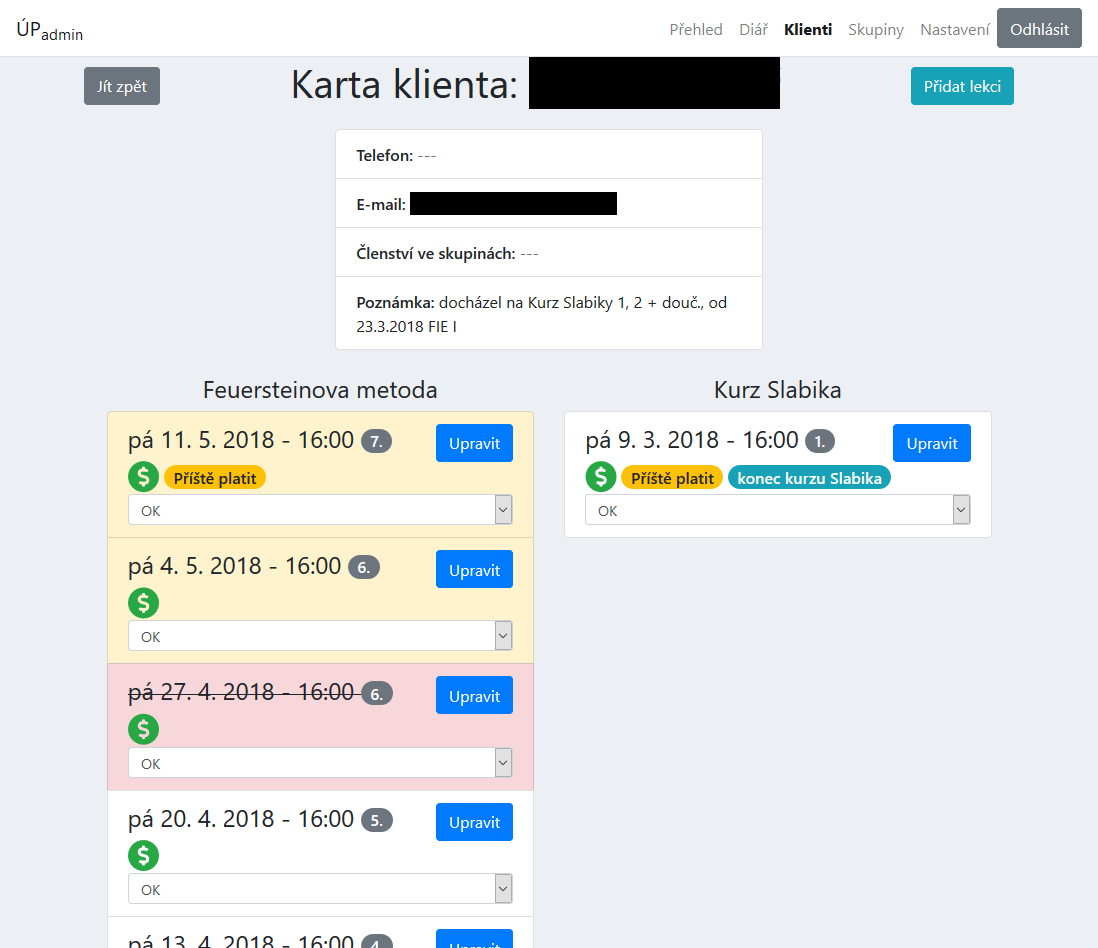
\includegraphics[width=1\textwidth]{img/screen-karta.png}
        	\caption{Snímek obrazovky s kartou klienta}\label{fig:screen-karta}
        \end{figure}
    
    Na obrázku~\ref{fig:screen-den} je ukázka přehledu pro aktuální den, toto je hlavní stránka aplikace, která se zobrazí po přihlášení. Lektorka zde vidí veškeré informace k lekcím na aktuální den a jednoduše může jedním kliknutím změnit stav účasti klientů či platbu (po provedení se zobrazí barevná notifikace s výsledkem operace), případně otevřít kartu klienta nebo skupiny. Bíle jsou individuální lekce, šedou barvou jsou zvýrazněny skupinové lekce.
    
        \begin{figure}[hb]\centering
        	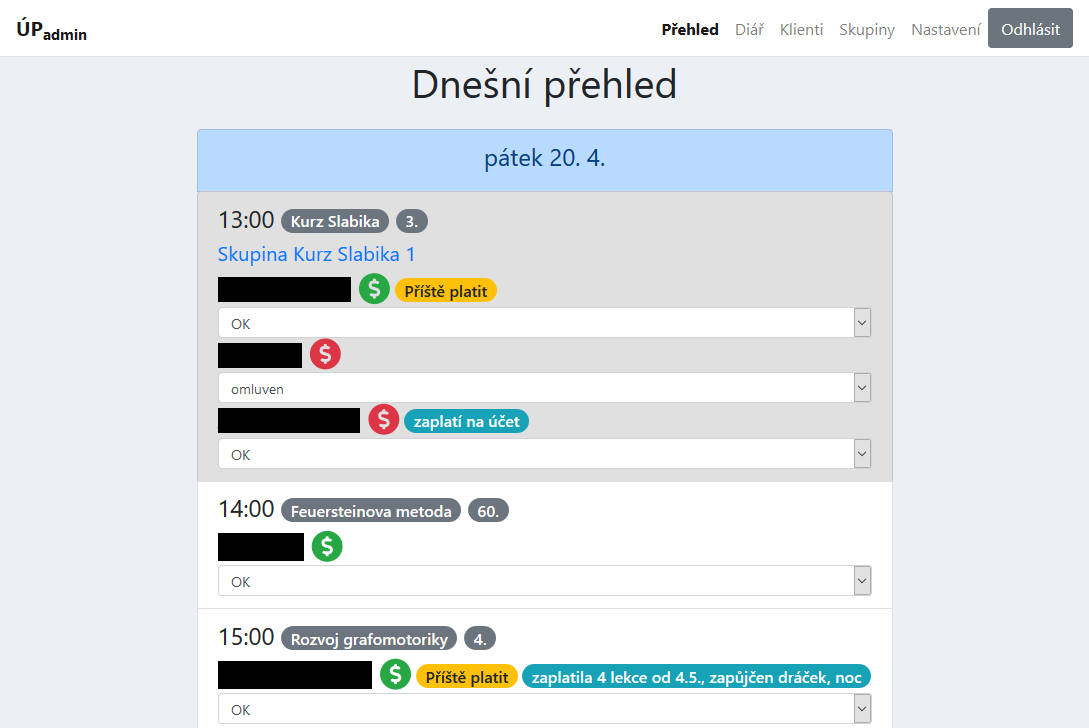
\includegraphics[width=1\textwidth]{img/screen-den.png}
        	\caption{Snímek obrazovky s denním přehledem}\label{fig:screen-den}
        \end{figure}
    
    Naprosto stejné prostředí nabízí týdenní přehled na obrázku~\ref{fig:screen-tyden} (je to dáno znovupoužitím stejné React komponenty), zde je vidět kromě již zmíněných prvků v denním přehledu modře zvýrazněný aktuální den v záhlaví příslušného dne, díky navigaci v horní části stránky lze bez znovunačítání stránky přecházet mezi jednotlivými týdny a vracet se jedním kliknutím na aktuální týden (tlačítko \enquote{Dnes}).
        
        \begin{landscape}
            \begin{figure}\centering
            	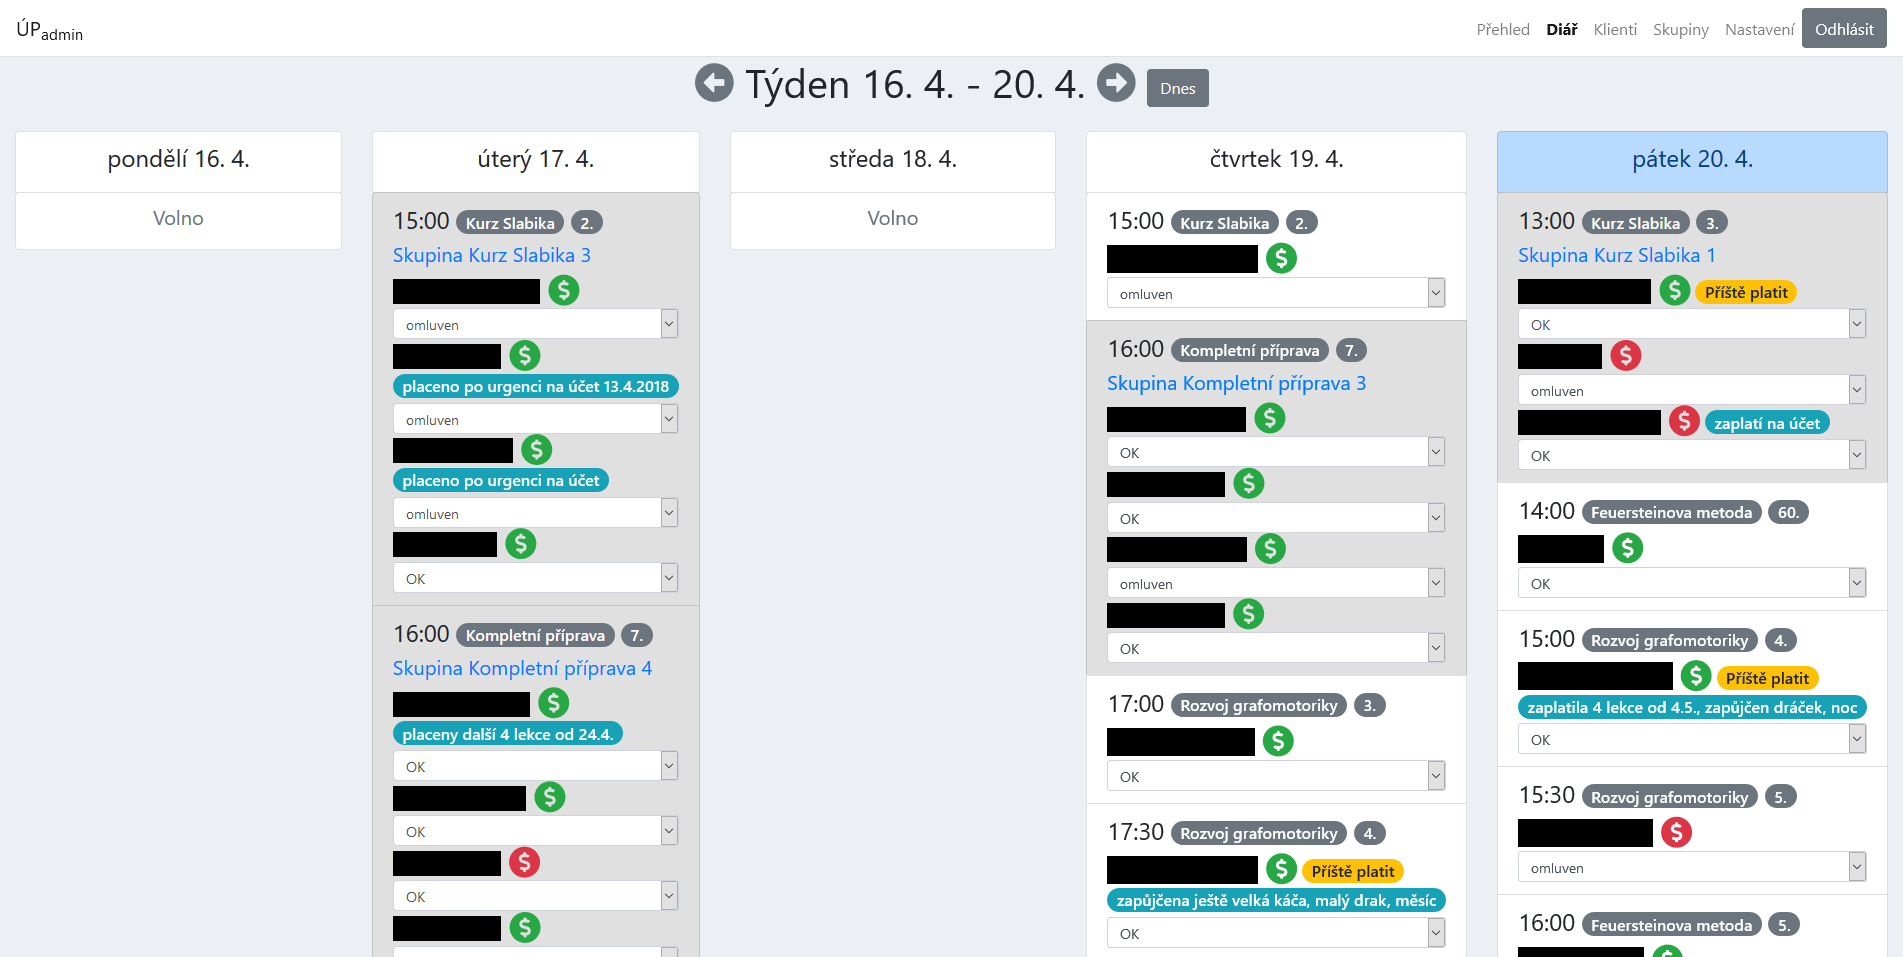
\includegraphics[totalheight=0.8\textheight]{img/screen-tyden.png}
            	\caption{Snímek obrazovky s týdenním přehledem}\label{fig:screen-tyden}
            \end{figure}
        \end{landscape}
    

\chapter{Další možná rozšíření}\label{dalsirozsireni}
Vytvořená aplikace je základem ÚP a už teď jsou ve fázi plánů a návrhů další funkcionality, které jsou potřeba. Týkají se jak doplnění funkcí do stávající evidence kurzů, lekcí, klientů a skupin, tak rozšíření aplikace o další části. Cílem této krátké kapitoly je nastínit plánovaná a možná rozšíření.

Co se týče stávajících funkcí, v nejbližší době je v plánu vylepšení funkcionality předplacených kurzů, rodiče totiž čím dál více volí možnost předplacení na mnoho lekcí dopředu a je potřeba umožnit jejich pohodlnější zaznamenání. Toto vylepšení také umožní vytvořit pohodlnější způsob evidence předplacených lekcí skupin, v současné době je to sice možné, ale ne úplně pohodlné. Dále je v plánu kontrola překryvu kurzů, tedy ochrana proti tomu, aby např. nenastal konflikt dvou lekcí v jeden čas. Také se počítá s přidáním vyhledávání do aplikace, díky kterému by bylo možné klienty a další objekty (např. pomůcky, viz. dále) snadno vyhledávat.

Mezi další funkce, které v budoucnu rozšíří působnost aplikace do dalších částí projektu, patří evidování zájemců o kurz -- například skupinové kurzy totiž většinou vznikají tak, že se vytvoří skupina zájemců a když se uvolní blok v týdnu a hodí se klientům z této skupiny, začnou lekce -- je tedy potřeba evidovat, kteří rodiče mají zájem o příslušný kurz a po domluvě umožnit vytvoření prvních lekcí. Také je v plánu vytvoření úplně nové části této aplikace pro evidenci pomůcek a učebnic, která je také mírně specifická a mimo tuto evidenci je potřeba její část napojit také na web. Dalším důležitým bodem ve vývoji aplikace je doplnění dalších testů a vysoké pokrytí kódu.

Jak jsem již zmínil v podsekci~\ref{sec:zakladniPraceSReactem}, během vývoje došlo k vydání nové verze Reactu, ruku v ruce s již zmíněnými rozšířeními je v plánu analýza možností využití nového Context API v Reactu, protože existují části aplikace, které by se dle mého názoru daly použitím tohoto API pravděpodobně vylepšit (např. snížení počtu přístupů do REST API). Stejně tak bude potřeba nadále držet krok s novějšími verzemi Reactu a přizpůsobit se tak novému životnímu cyklu komponent a případně dalším změnám.

Mezi další nápady na vylepšení je zpřístupnění údajů offline, bude tedy potřeba prozkoumat možnosti řešení jako např. automatické ukládání do Google kalendáře, progresivní webové aplikace apod. a s tím související další oblasti jako SSR (viz. podsekce~\ref{client-side-scripting}).

Takto rozšířená aplikace tak ještě více urychlí a zefektivní každodenní práci a pomůže tak lektorce získat další čas pro samotné lekce, jejich přípravu a rozvoj.